%%%%%%%%%%%%%%%%%%%%%%%%%%%%%%%%%%%%%%%%%
% Short Sectioned Assignment
% LaTeX Template
% Version 1.0 (5/5/12)
%
% This template has been downloaded from:
% http://www.LaTeXTemplates.com
%
% Original author:
% Frits Wenneker (http://www.howtotex.com)
%
% License:
% CC BY-NC-SA 3.0 (http://creativecommons.org/licenses/by-nc-sa/3.0/)
%
%%%%%%%%%%%%%%%%%%%%%%%%%%%%%%%%%%%%%%%%%

%----------------------------------------------------------------------------------------
%	PACKAGES AND OTHER DOCUMENT CONFIGURATIONS
%----------------------------------------------------------------------------------------

\documentclass[paper=a4, fontsize=11pt]{scrartcl} % A4 paper and 11pt font size

\usepackage[T1]{fontenc} % Use 8-bit encoding that has 256 glyphs
\usepackage{fourier} % Use the Adobe Utopia font for the document - comment this line to return to the LaTeX default
\usepackage[english]{babel} % English language/hyphenation
\usepackage{amsmath,amsfonts,amsthm} % Math packages

\usepackage{lipsum} % Used for inserting dummy 'Lorem ipsum' text into the template

\usepackage{sectsty} % Allows customizing section commands
\allsectionsfont{\centering \normalfont\scshape} % Make all sections centered, the default font and small caps

\usepackage{fancyhdr} % Custom headers and footers
\pagestyle{fancyplain} % Makes all pages in the document conform to the custom headers and footers
\fancyhead{} % No page header - if you want one, create it in the same way as the footers below
\fancyfoot[L]{} % Empty left footer
\fancyfoot[C]{} % Empty center footer
\fancyfoot[R]{\thepage} % Page numbering for right footer
\renewcommand{\headrulewidth}{0pt} % Remove header underlines
\renewcommand{\footrulewidth}{0pt} % Remove footer underlines
\setlength{\headheight}{13.6pt} % Customize the height of the header

\numberwithin{equation}{section} % Number equations within sections (i.e. 1.1, 1.2, 2.1, 2.2 instead of 1, 2, 3, 4)
\numberwithin{figure}{section} % Number figures within sections (i.e. 1.1, 1.2, 2.1, 2.2 instead of 1, 2, 3, 4)
\numberwithin{table}{section} % Number tables within sections (i.e. 1.1, 1.2, 2.1, 2.2 instead of 1, 2, 3, 4)

\setlength\parindent{0pt} % Removes all indentation from paragraphs - comment this line for an assignment with lots of text

\usepackage{graphicx}
\usepackage{caption}
\usepackage{subcaption}
%----------------------------------------------------------------------------------------
%	TITLE SECTION
%----------------------------------------------------------------------------------------

\newcommand{\horrule}[1]{\rule{\linewidth}{#1}} % Create horizontal rule command with 1 argument of height

\title{	
\normalfont \normalsize 
\textsc{University of California San Diego} \\ [25pt] % Your university, school and/or department name(s)
\horrule{0.5pt} \\[0.4cm] % Thin top horizontal rule
\huge CSE 260 -- Parallel Computation \\ Programming Lab 2 \\ High Performance Matrix Multiplication\\on a GPU\\ Group ID: G-418-960 % The assignment title
\horrule{2pt} \\[0.5cm] % Thick bottom horizontal rule
}

\author{Andreas Prodromou, Samuel Wasmundt \\ <A530-492-30>, <A530-537-28>} % Your name

\date{\normalsize\today} % Today's date or a custom date

\begin{document}

\maketitle % Print the title

%----------------------------------------------------------------------------------------
%	PROBLEM 1
%----------------------------------------------------------------------------------------

\begin{abstract}
For this project we modified the files mmpy.cu, genMatrix.cpp, and mmpy\_kernel.cu. We implemented each optimization as a separate function in order to allow for better evaluation, thus we had to modify mmpy.cu in order to be able to select the correct kernel according to a compilation flag. The genMatrix was modified in order to allow us to generate a transposed matrix for the cases were matrix B had to be transposed for our optimizations to work. If these files are taken from our Turnin repository, a normal ``make'' command will produce the most optimized executable.
\end{abstract}

\section{\textbf{High Performance Matrix Multiplication on a GPU}}

The goal of this project was to optimize matrix multiplication for NVIDIA's Fermi GPU. Our starting point was a naive CUDA implementation. Performance throughout this document is reported on the Dirac platform located at NERSC. On Dirac, our code is executed on Tesla C2050 GPUs.\\

A total of six optimizations were attempted by our group, all building on top of the naive code provided. Specifically the optimizations we implemented include:

\begin{enumerate}
\item Tiling for improved computation ratio
\item Memory coalescing
\item Avoiding memory bank conflicts
\item Reducing the number of instructions with multiply add balancing
\item Prefetching
\item Loop unrolling
\end{enumerate}

Throughout this report, we describe the details for each of these optimizations and how they were implemented. We report the performance improvement observed after their implementation. Figures \ref{fig:multi1} and \ref{fig:multi2} display an overview of each optimization and its impact on the overall performance. In these four figures, we are reporting all the results obtained from our study. Thread blocks with geometries of 16$\times$16 and 32$\times$32 and both single and double precision floating point matrices. We should note that the last three optimizations have a different grid geometry than the rest. The reason will be explained later in this document.

\begin{figure} [h]
\centering
\begin{subfigure}{.5\textwidth}
  \centering
  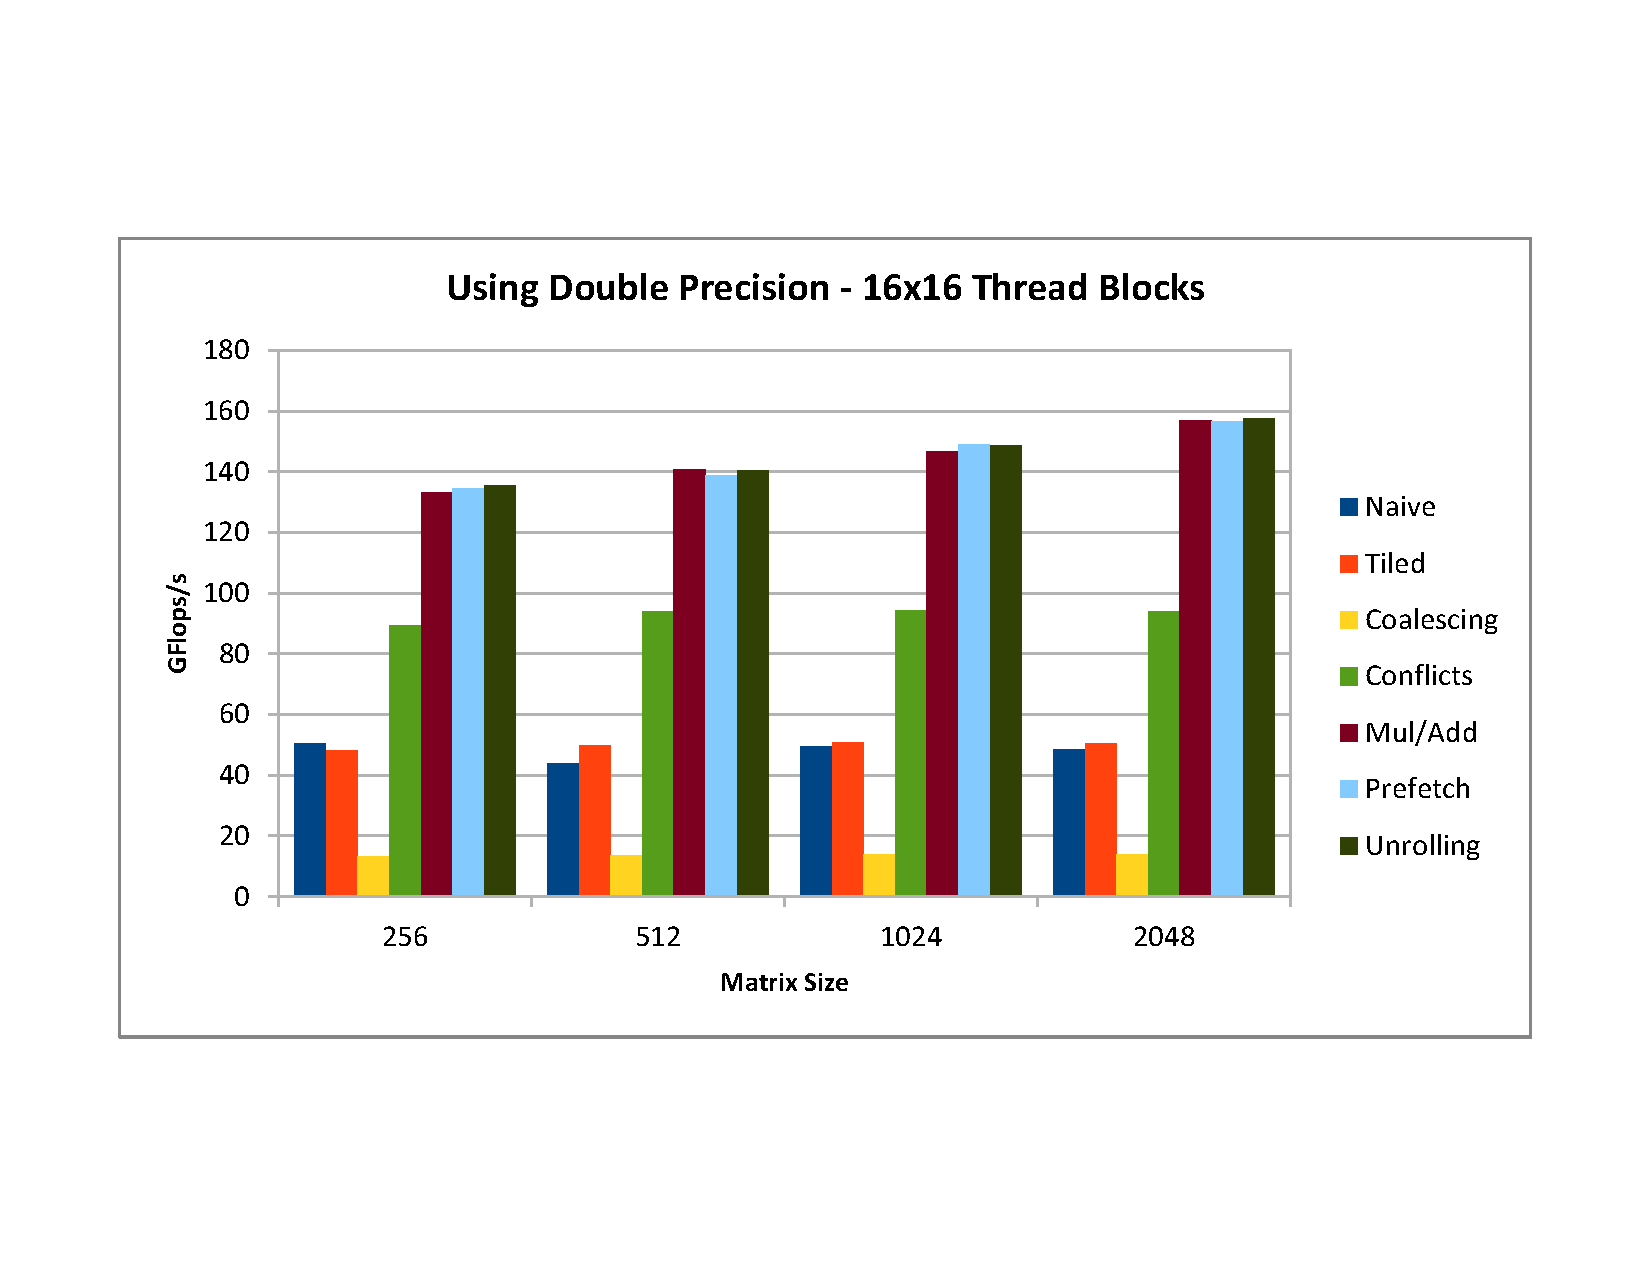
\includegraphics[width=1.07\linewidth]{figures/all_Double_16.pdf}
  \label{fig:all_double_16}
\end{subfigure}%
\begin{subfigure}{.5\textwidth}
  \centering
  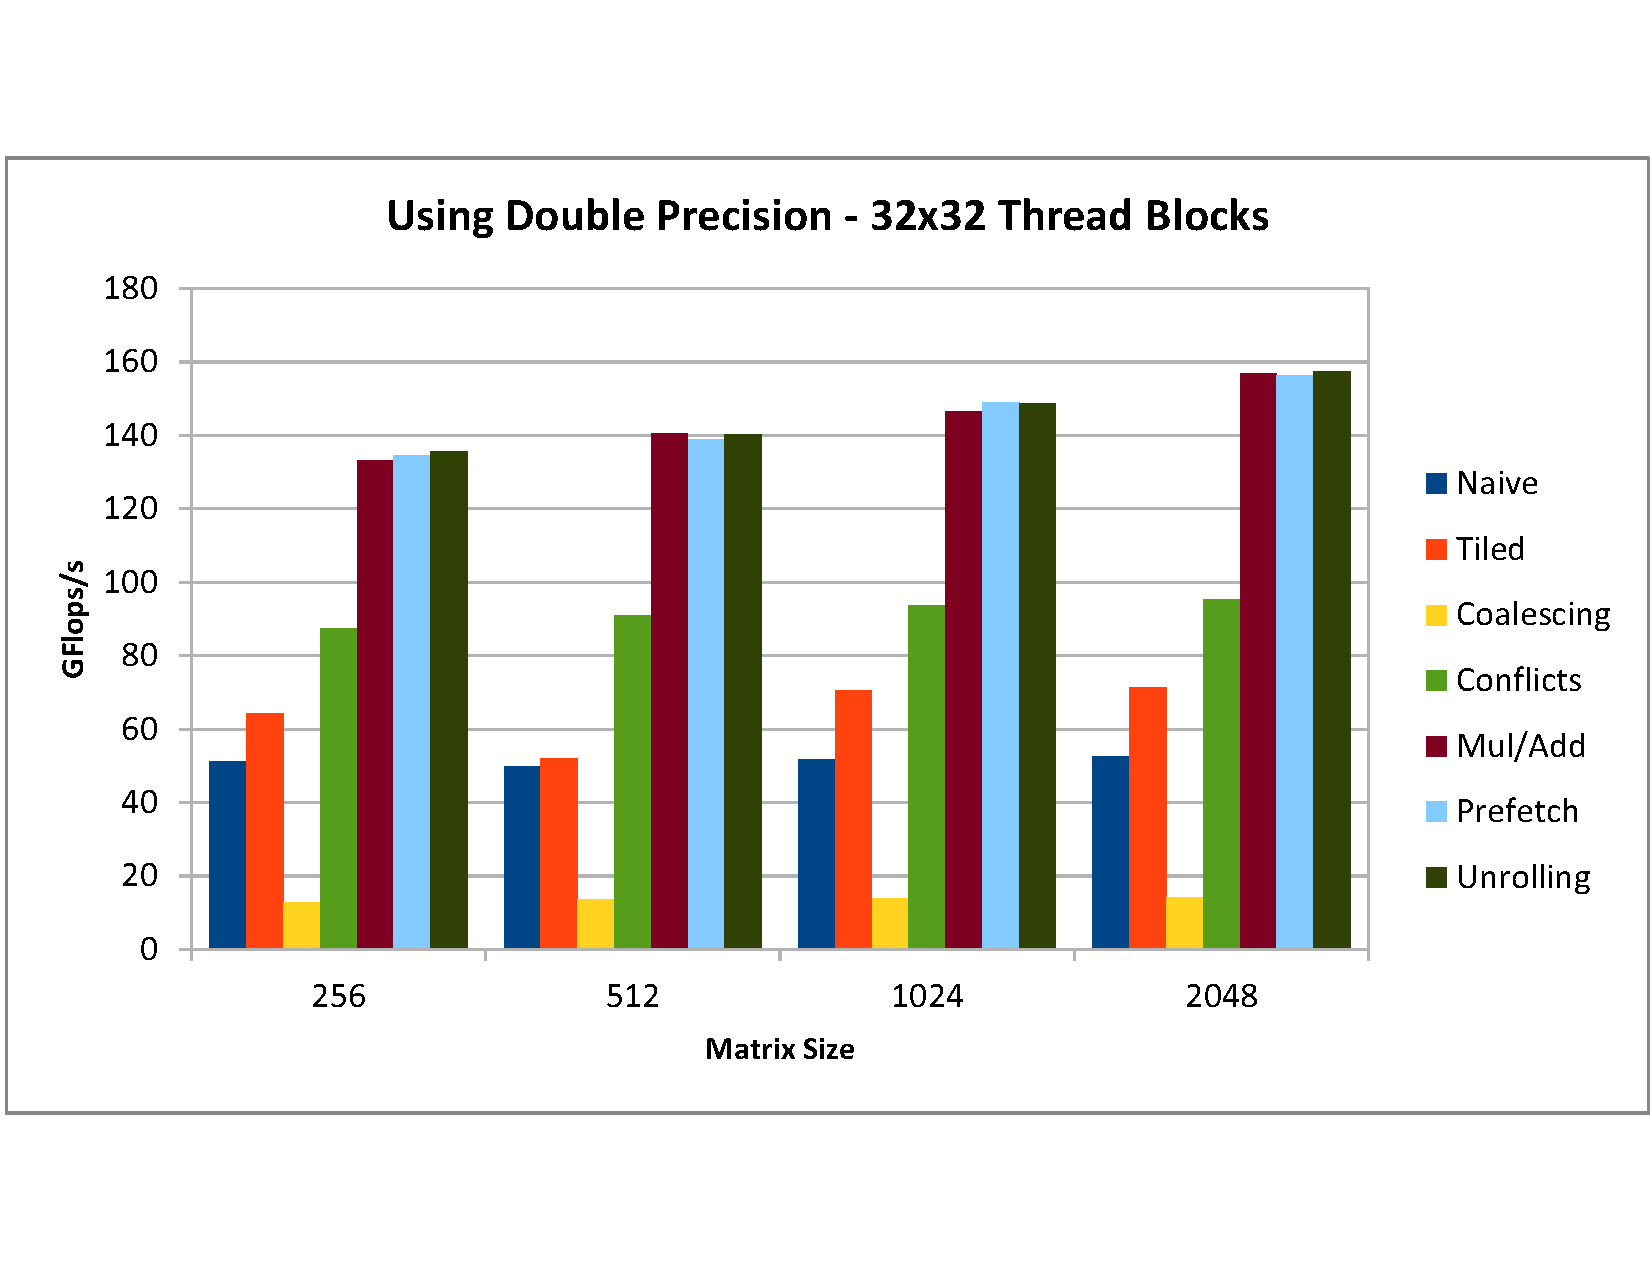
\includegraphics[width=\linewidth]{figures/all_Double_32.pdf}
  \label{fig:all_double_32}
\end{subfigure}
\caption{Double Precision Arithmetic Used. The left figure presents the performance of 16$\times$16 thread blocks, while the right figure uses 32$\times$32 thread blocks.}
\label{fig:multi1}
\end{figure}

\begin{figure} [h]
\centering
\begin{subfigure}{.5\textwidth}
  \centering
  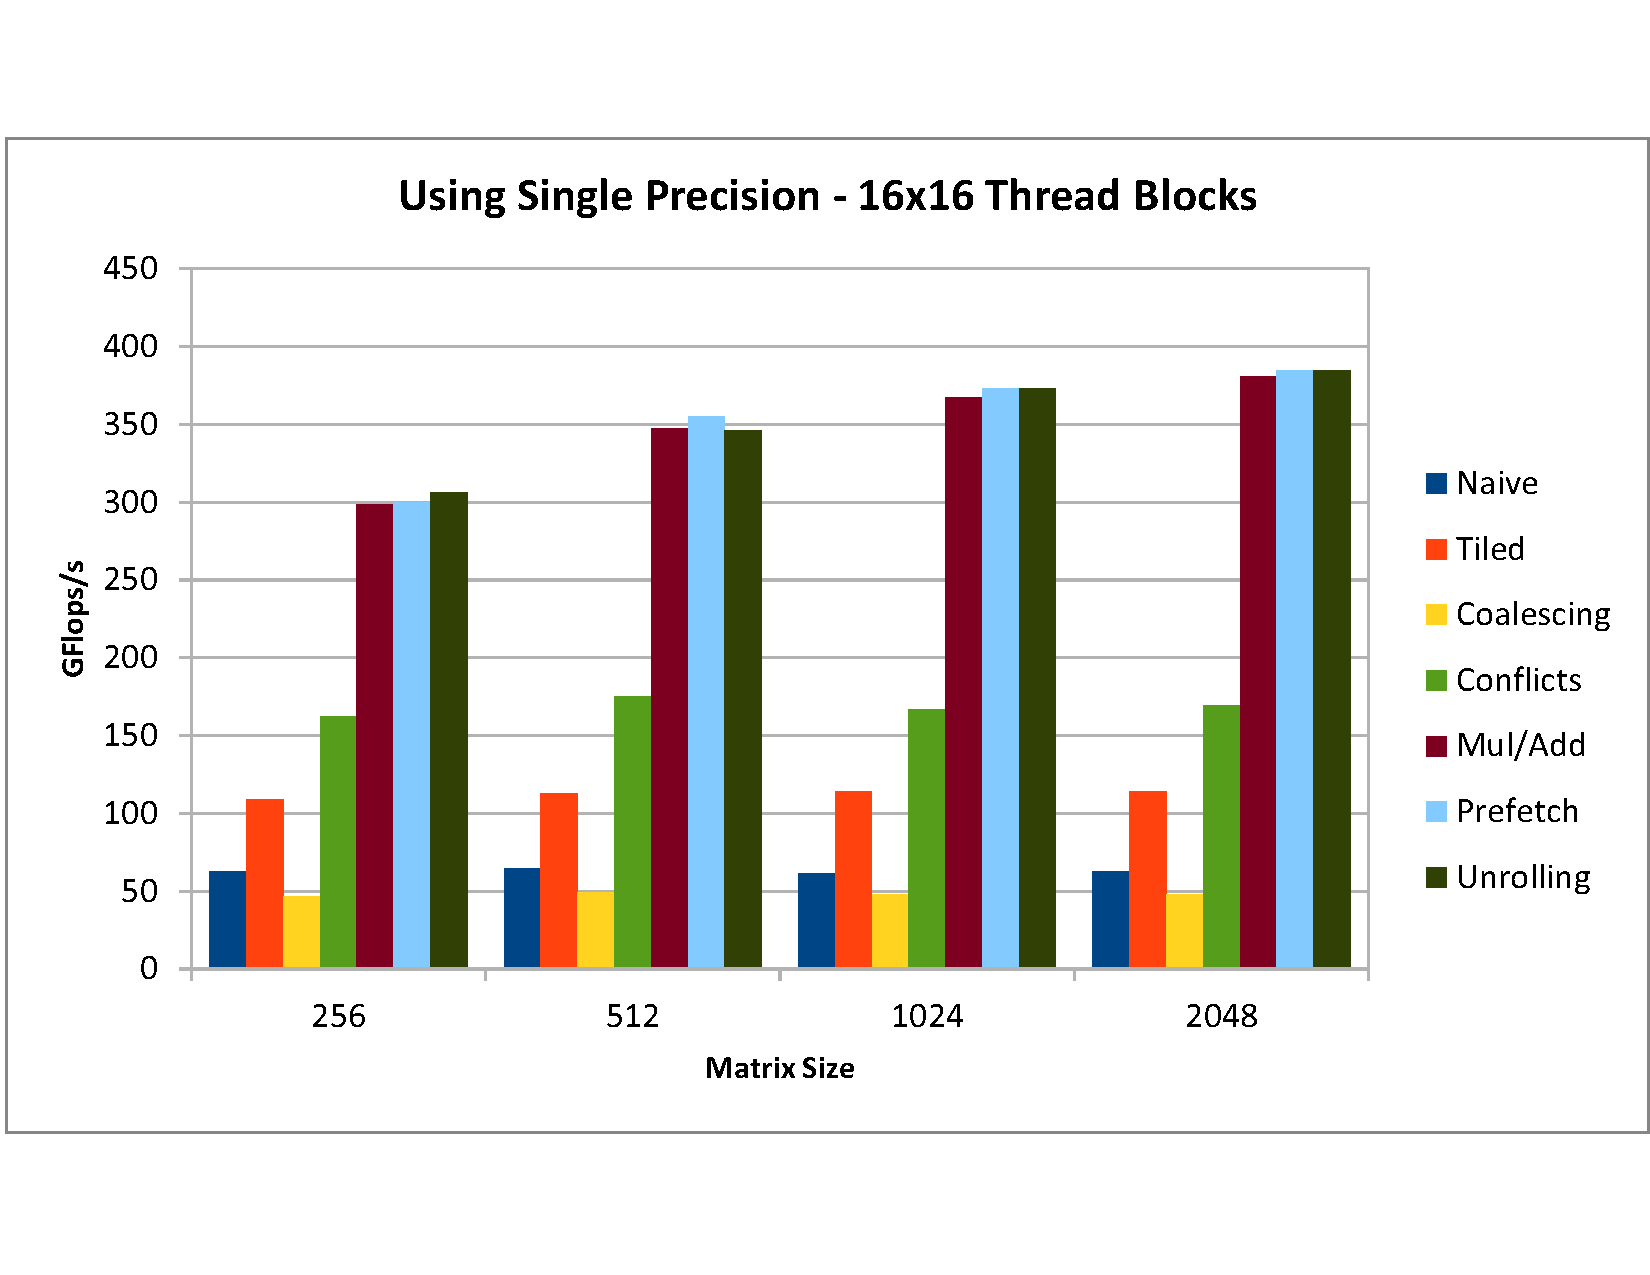
\includegraphics[width=2.85in]{figures/all_Single_16.pdf}
  \label{fig:all_single_16}
\end{subfigure}%
\begin{subfigure}{.5\textwidth}
  \centering
  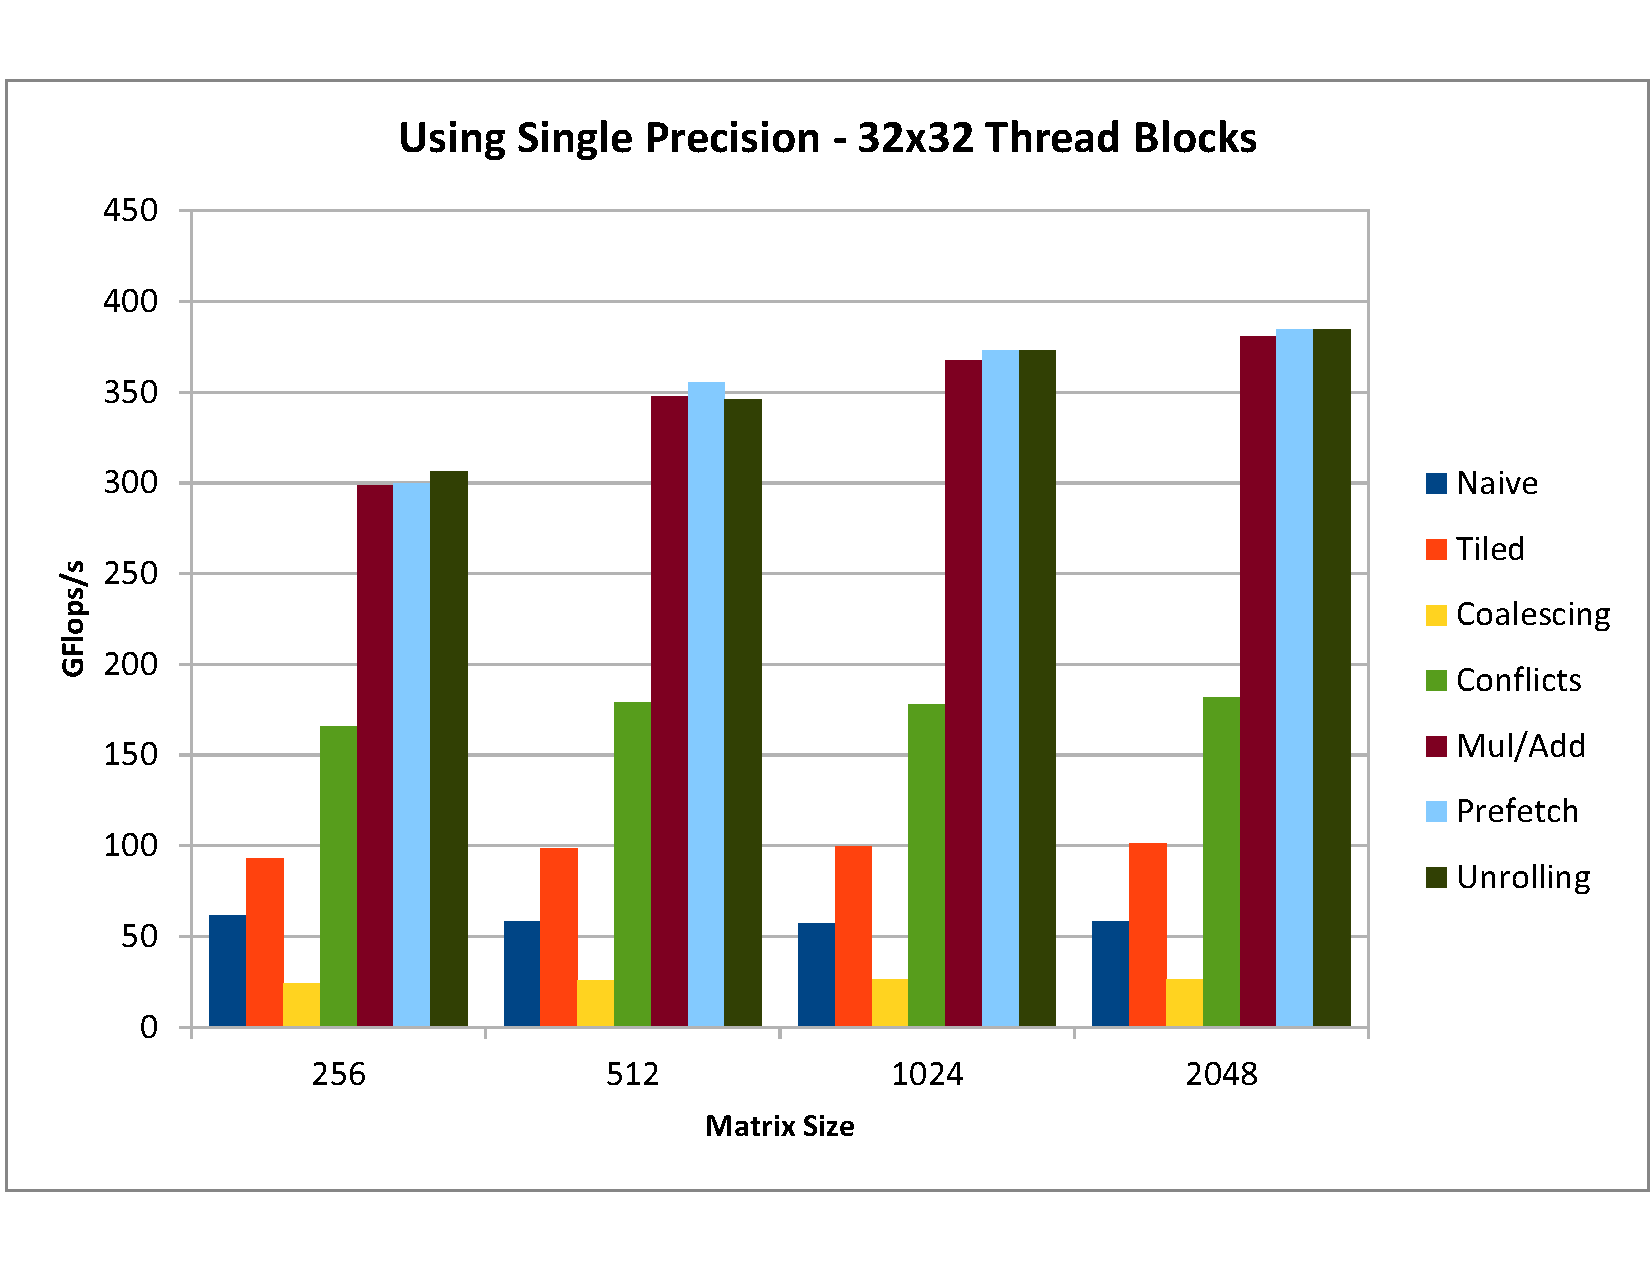
\includegraphics[width=2.6in]{figures/all_Single_32.pdf}
  \label{fig:all_single_32}
\end{subfigure}
\caption{Single Precision Arithmetic Used. The left figure presents the performance of 16$\times$16 thread blocks, while the right figure uses 32$\times$32 thread blocks.}
\label{fig:multi2}
\end{figure}

\section{\textbf{Multicore Implementation}}
Part of the provided code, was a multicore implementation of matrix multiplication, using MPI. This code was compiled and executed on Dirac, using 8 threads (we set the OMP\_NUM\_THREADS variable to 8).\\

To get a good measurement for this algorithm's performance, we performed a series of tests, ranging the input size from  128 to 2048 with power-of-2 increments, ten repetitions in each execution and we also ran multiple executions. The peak performance measurement for the multicore algorithm was obtained for input size of 1024 and specifically 28.94 GFlops/s. \\

We can observe that even the naive CUDA implementation performs significantly better than the multicore one and the reason is the higher amount of parallelization that can be extracted from the GPU comparative to the CPU core. For the rest of this document, we will be reporting our results in comparison to the naive CUDA implementation.

\section{\textbf{Naive Implementation}}
The naive kernel was part of the provided source code. In this kernel, each thread computes one element (cell) of the result matrix, by getting a row of the A matrix, a column of the B matrix and computing the inner product. Figure \ref{fig:naive} demonstrates the performance of the naive algorithm on Dirac, for matrix sizes of 256, 512, 1024 and 2048. We also display the corresponding performance measurements for single precision floating point numbers under the same kernel.\\

\begin{figure}[h]
  \centering
    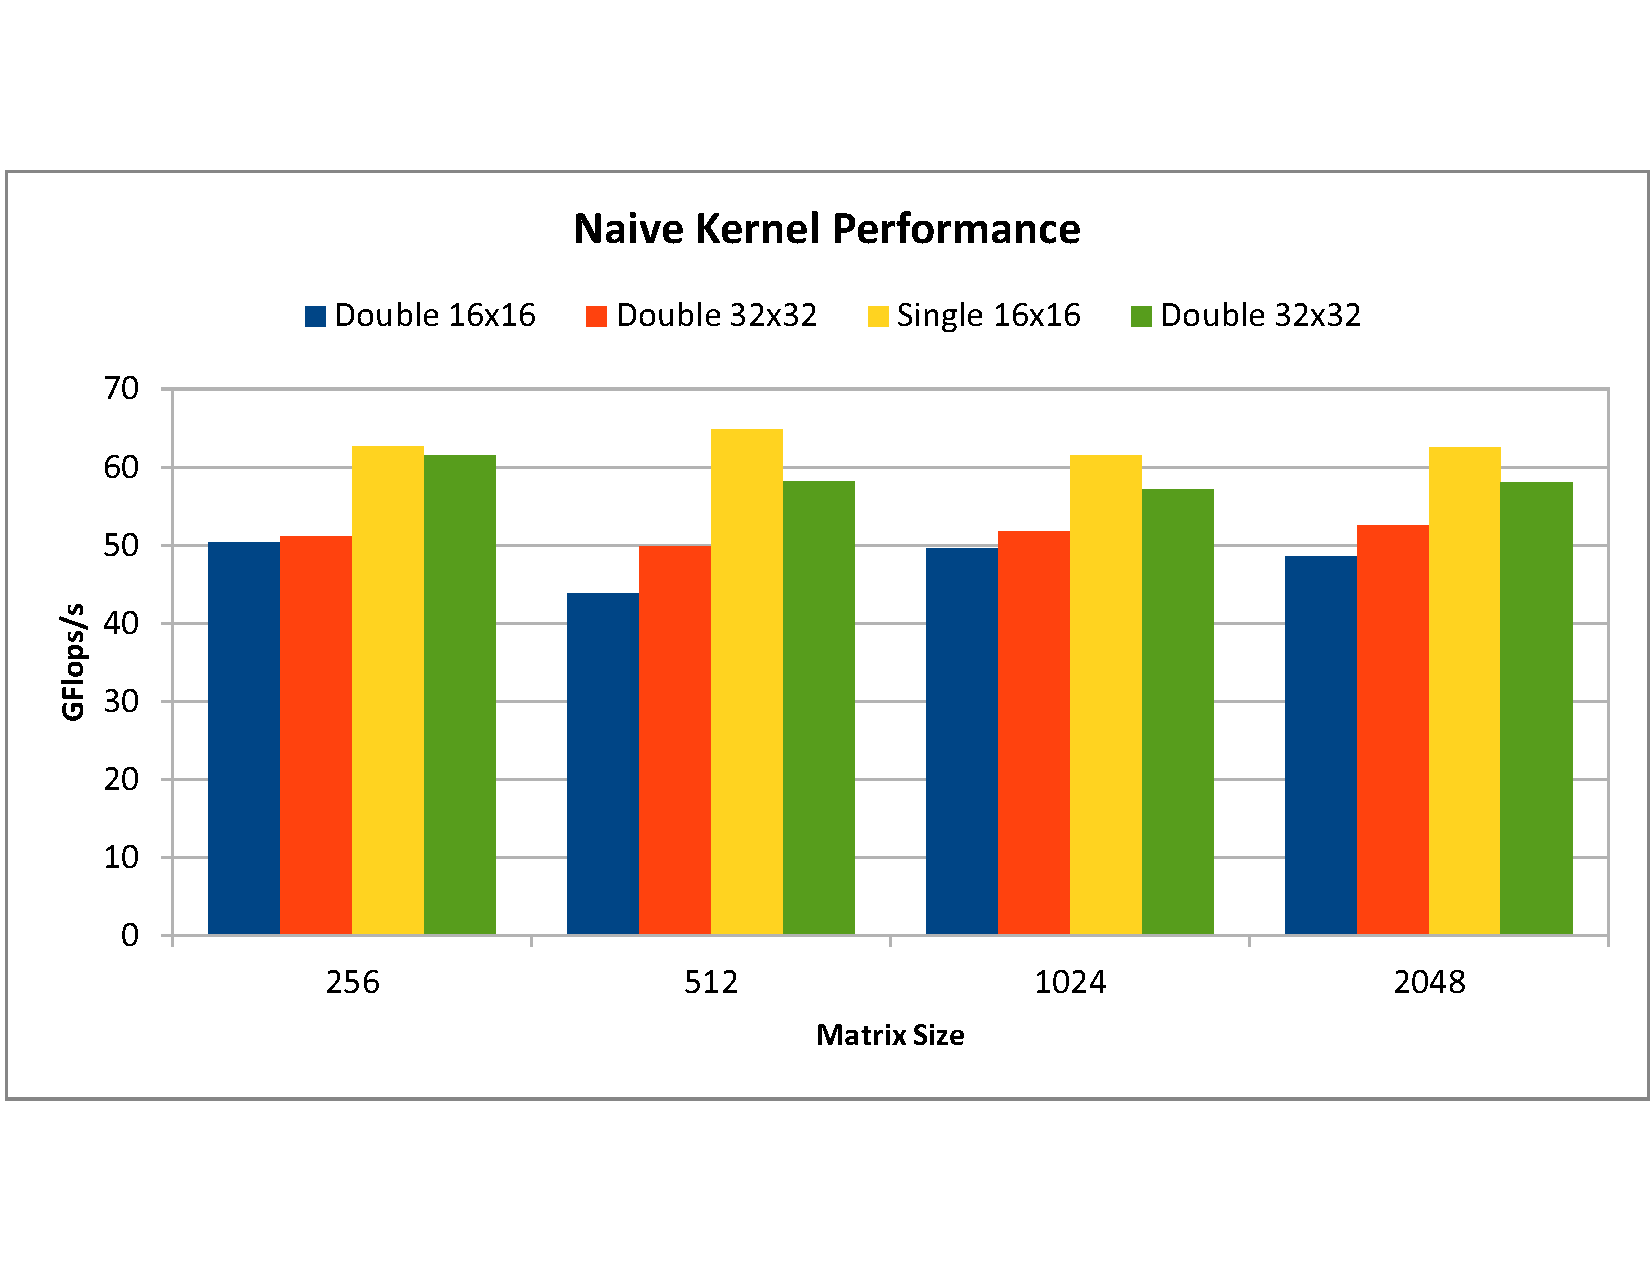
\includegraphics[width=0.8\textwidth]{figures/naive.pdf}
    \caption{Naive algorithm's Performance}
    \label{fig:naive}
\end{figure}

The first column in the Figure shows the performance of thread blocks with 16x16 threads on double values. The second still uses double values but 32x32 thread blocks. Similarly -- but with single values -- the third and fourth column use 16x16 and 32x32 thread blocks respectively.\\

Examining the naive implementation when executing double precision floating point matrix multtiplication, we can see that the amount of computations performed is in the order of N$^3$, where N$^2$ is the size of each matrix. If we calculate the number of memory accesses, N$^3$ double precision values (8 bytes) need to be accessed. Essentially, the naive code does one floating-point operation (flop) per 8 bytes.

\section{\textbf{Tiling for Improved computation Ratio}}

The naive implementation is clearly memory bounded, so this first optimization attempts to re-use values in order to reduce the computation-memory ratio. As performed in the first assignment of this class, tiling allows this re-use and is a good candidate for a first optimization. In the first assignment, tiling was performed in order to fit as many values as possible in the processor's cache, thus improving the performance.\\ 

Similarly, when programming in CUDA, tiling will bring useful values into the GPU's shared memory. In the naive case, the matrices were kept in the global memory which is slower. The idea of tiling is simple; Divide the matrices into tiles and have each thread block perform a fraction of the overall calculation required for C (the result matrix).\\

In other words, each thread block loads a block of A and a block of B into shared memory and then performs matrix multiplication on the smaller blocks. Since each thread block is responsible for a matrix block (tile), the block's geometry is correlated with the blocking size. For example, if we want to perform tiling with 32$\times$32 tile size, we need 32$\times$32 threads in each block.\\

\begin{figure} [h]
\centering
\begin{subfigure}{.5\textwidth}
  \centering
  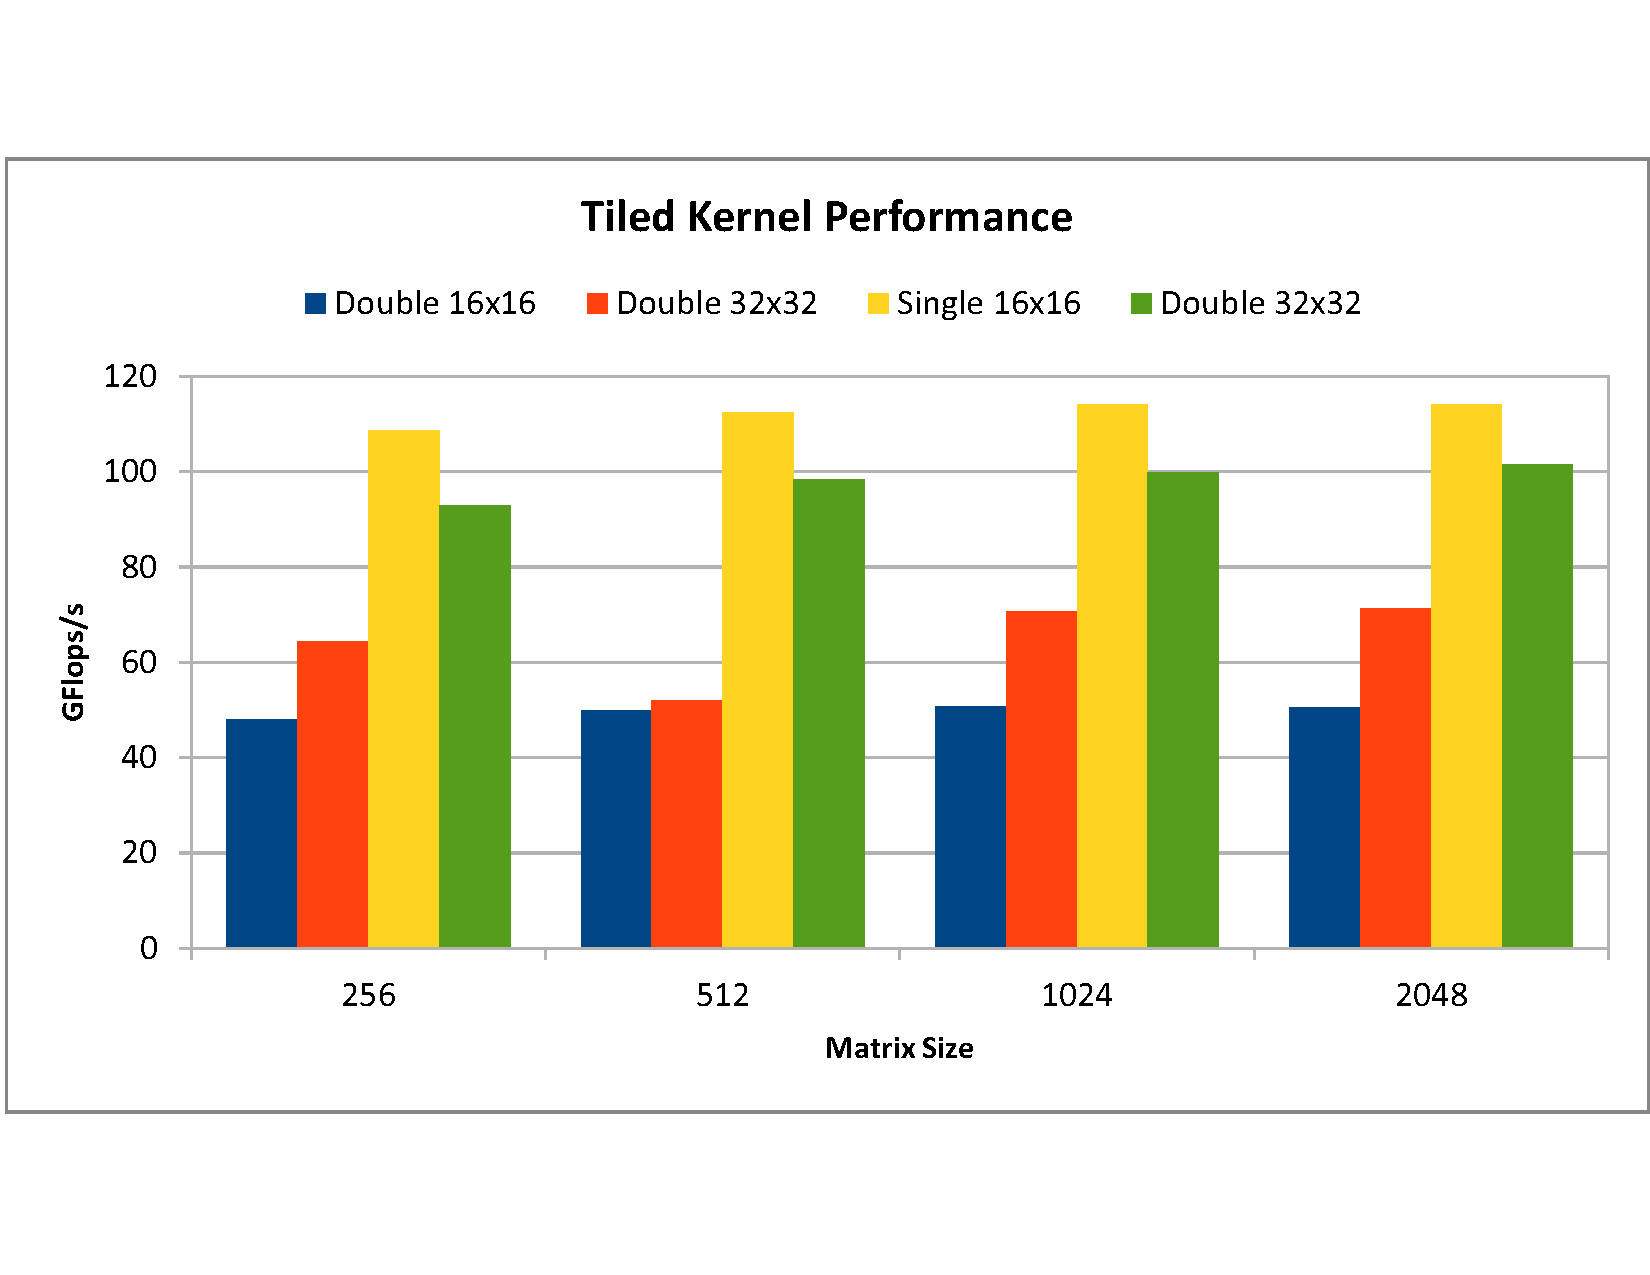
\includegraphics[width=\linewidth]{figures/tiled.pdf}
  \label{fig:tiled}
\end{subfigure}%
\begin{subfigure}{.5\textwidth}
  \centering
  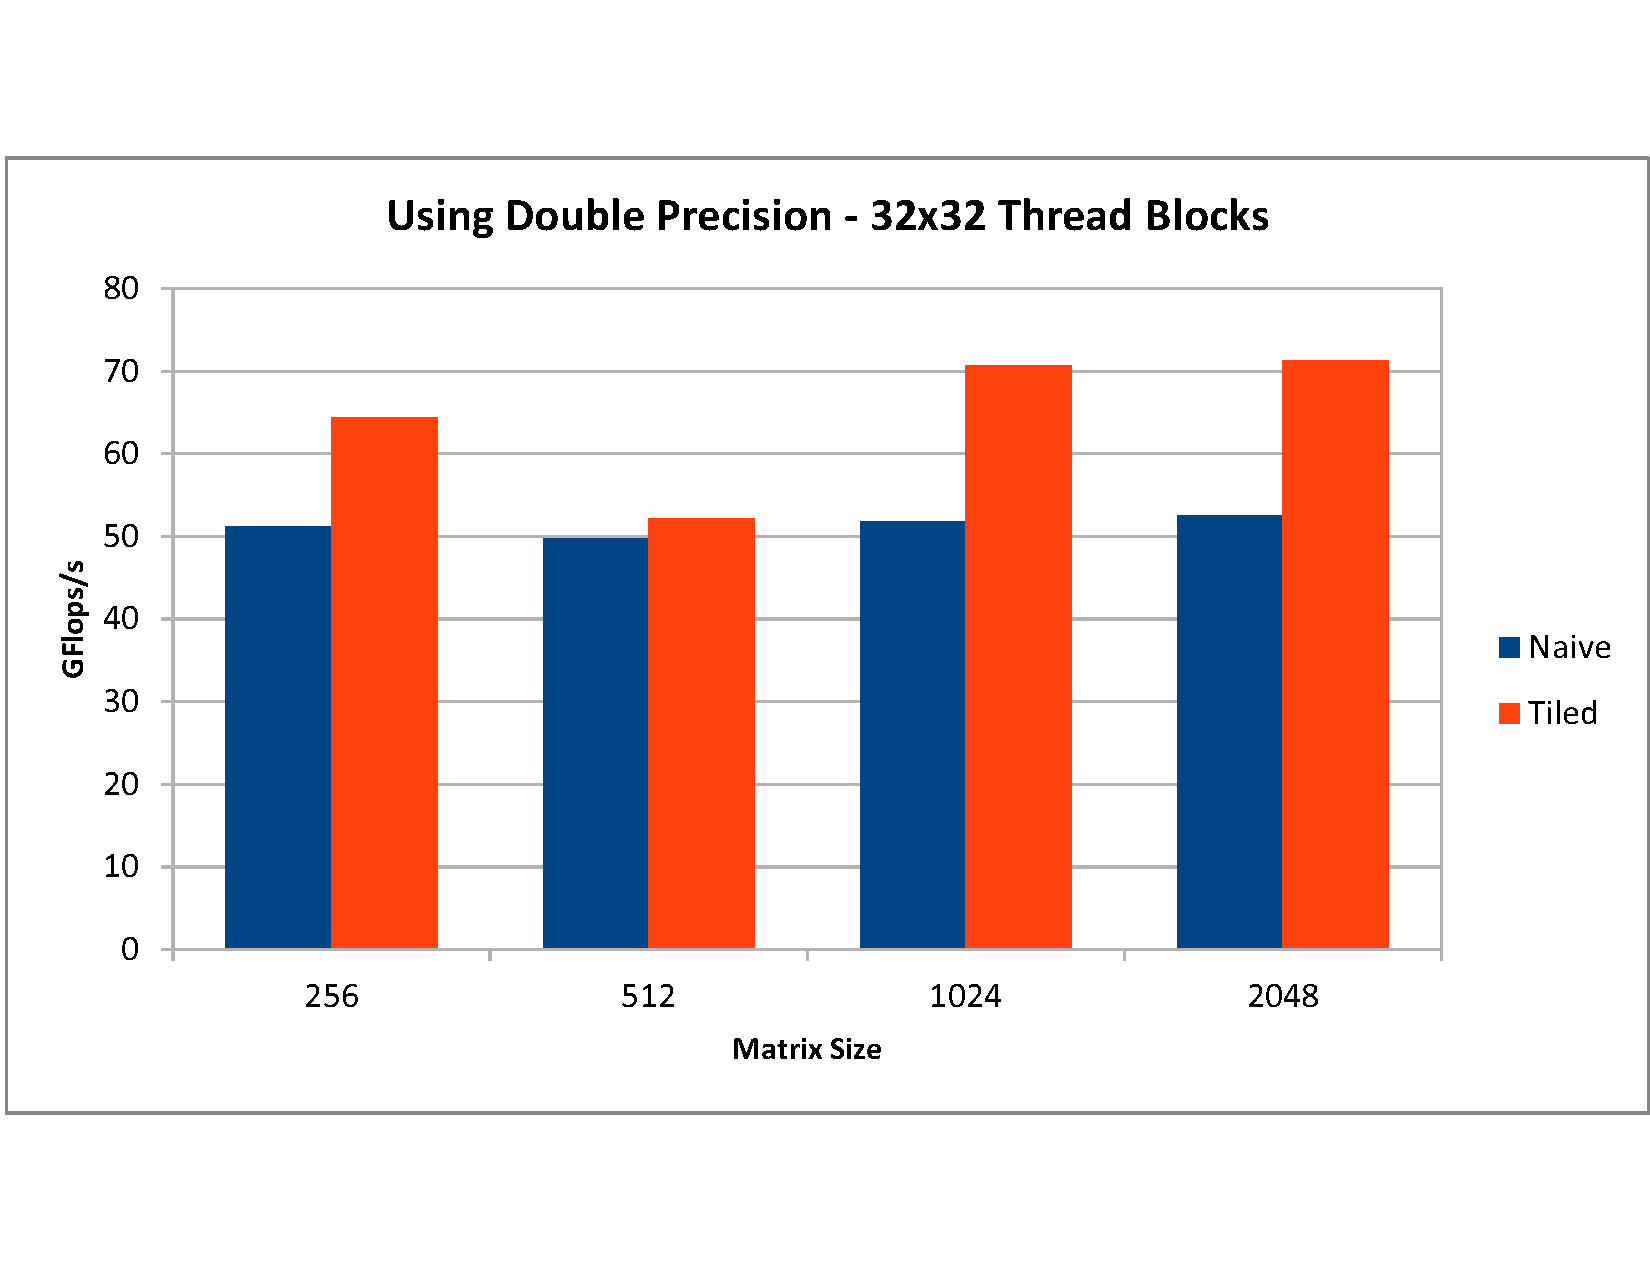
\includegraphics[width=\linewidth]{figures/tiled_vs_naive.pdf}
  \label{fig:tiled_vs_naive}
\end{subfigure}
\caption{Left: The performance of the Tiled Kernel. Right: Tiled kernel compared against the naive implementation.}
\label{fig:multi3}
\end{figure}

A consequence of tiling is that the code now only works with matrices with a size divisible by the block size. For this report, we are dealing with matrices of size 256, 512, 1024 and 2048, which all fall into the ``accepted'' category. For the remaining matrix sizes, we could increase the size of the input to an acceptable size and pad the new slots with zeros. This way we would be able to perform the multiplication on any arbitrary sized input.\\

Figure \ref{fig:multi3} (left) shows the performance measurements for this optimization for block sizes 32$\times$32 and 16$\times$16, and both double and single precision numbers. Figure \ref{fig:multi3} (right) displays the comparison between the tiled kernel and the naive one. We can see how performance is significantly improved by tiling. Using tiling, the number of memory accesses is now reduced to N$^3$/BLOCK\_SIZE, for tiles of size BLOCK\_SIZE$\times$BLOCK\_SIZE. The computation ratio is now increased to BLOCK\_SIZE flops per 8 bytes.

\section{\textbf{Memory Coalescing}}

Memory coalescing occurs when our code accesses the elements of an array stored in memory and these elements are stored in separate memory modules (banks). When memory is accessed in this way, subsequent reads are much faster than reading something from the same memory bank. In our case, the code is reading a line of A (matrix or sub-block) and a column of B. Reading the line of A creates coalesced memory accesses, however reading a column (i.e. stride = BLOCK\_SIZE) of B results in non-coalesced memory accesses, theoretically hurting performance.\\

To fix the coalescing issue, all we need to do is transpose B at the host before transferring it to the GPU. This way we can now read a row of A and a row of the transposed B matrix. The code for this coalesced kernel is very similar to the tiled kernel, with the exception of switching the indices when accessing B. In other words, we need to have B[i][j] instead of the old B[j][i]. We modified the genMatrix.cpp source file in order to create B transposed.\\

\begin{figure} [h]
\centering
\begin{subfigure}{.5\textwidth}
  \centering
  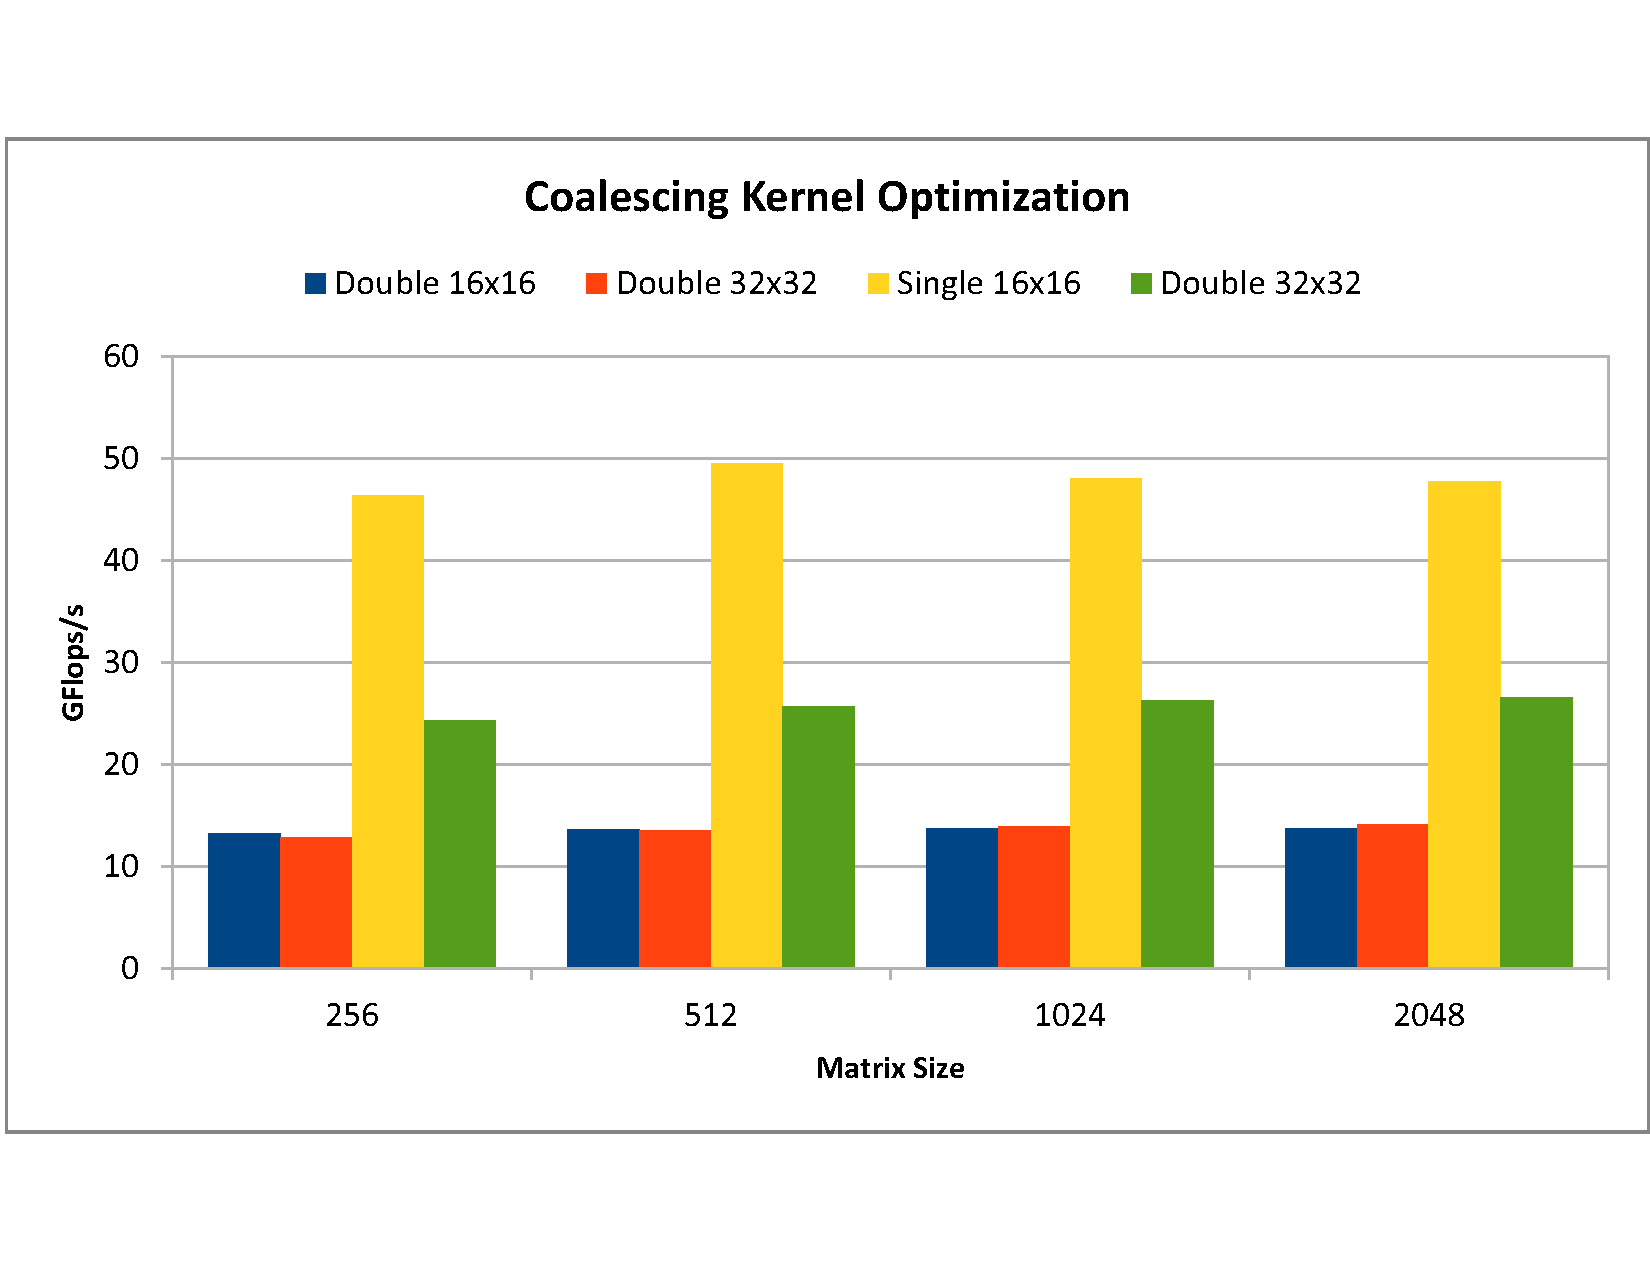
\includegraphics[width=\linewidth]{figures/coalescing.pdf}
  \label{fig:coalesced}
\end{subfigure}%
\begin{subfigure}{.5\textwidth}
  \centering
  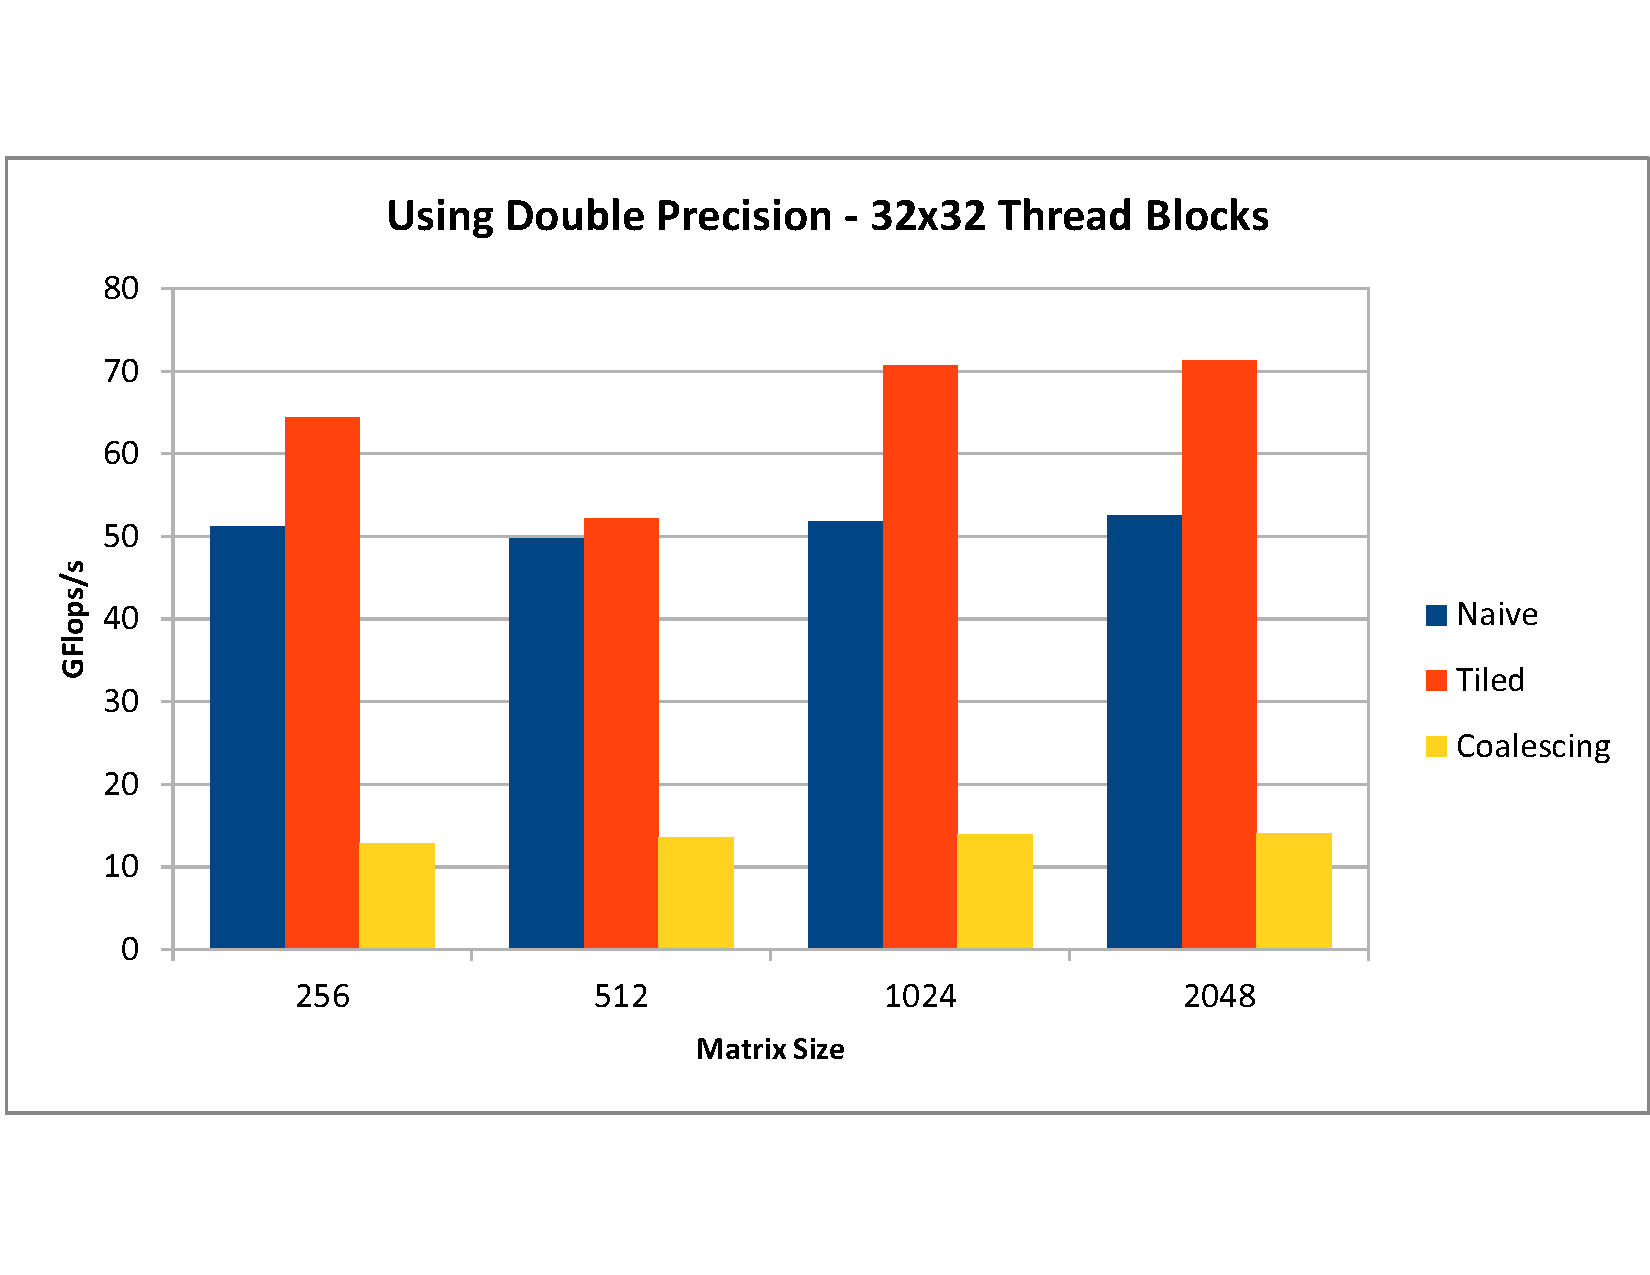
\includegraphics[width=1.03\linewidth]{figures/coalescing_vs_tiled.pdf}
  \label{fig:coalesced_vs_tiled}
\end{subfigure}
\caption{Left: The performance of the Memory Coalescing Kernel. Right: Memory Coalescing kernel compared against all previous optimizations.}
\label{fig:multi4}
\end{figure}

Figure \ref{fig:multi4} (left) displays the performance measured with this optimization (tiling is still performed) and Figure \ref{fig:multi4} (right) plots the performances of the naive, tiled and coalesced kernel. We observe a significant drop of performance when we use this optimization (even worst than the naive). As will be demonstrated in the next section, the reason is that when we perform coalesced memory accesses this way, we introduce a significant amount of bank conflicts, a factor which (as indicated by our results in the next section) plays a crucial role in the overall kernel performance.



\section{\textbf{Avoiding Memory Bank Conflicts}}
Memory bank conflicts occur when we are accessing memory locations of the same memory bank. Bank conflicts introduce a significant overhead and hurt performance. Even though the previous optimization manages to create coalesced accesses, each thread in the kernel loads an element of A into shared memory and then immediately the corresponding element of B \textit{from the same memory bank}. This results in a bank conflict on every thread's accesses to memory.\\

To overcome this issue, we programmed the kernel in such a way that each thread loads one element of A (say the first element) but then loads the last element of B instead of the first again. This way we don't introduce such a high amount of bank conflicts.\\

\begin{figure} [h]
\centering
\begin{subfigure}{.5\textwidth}
  \centering
  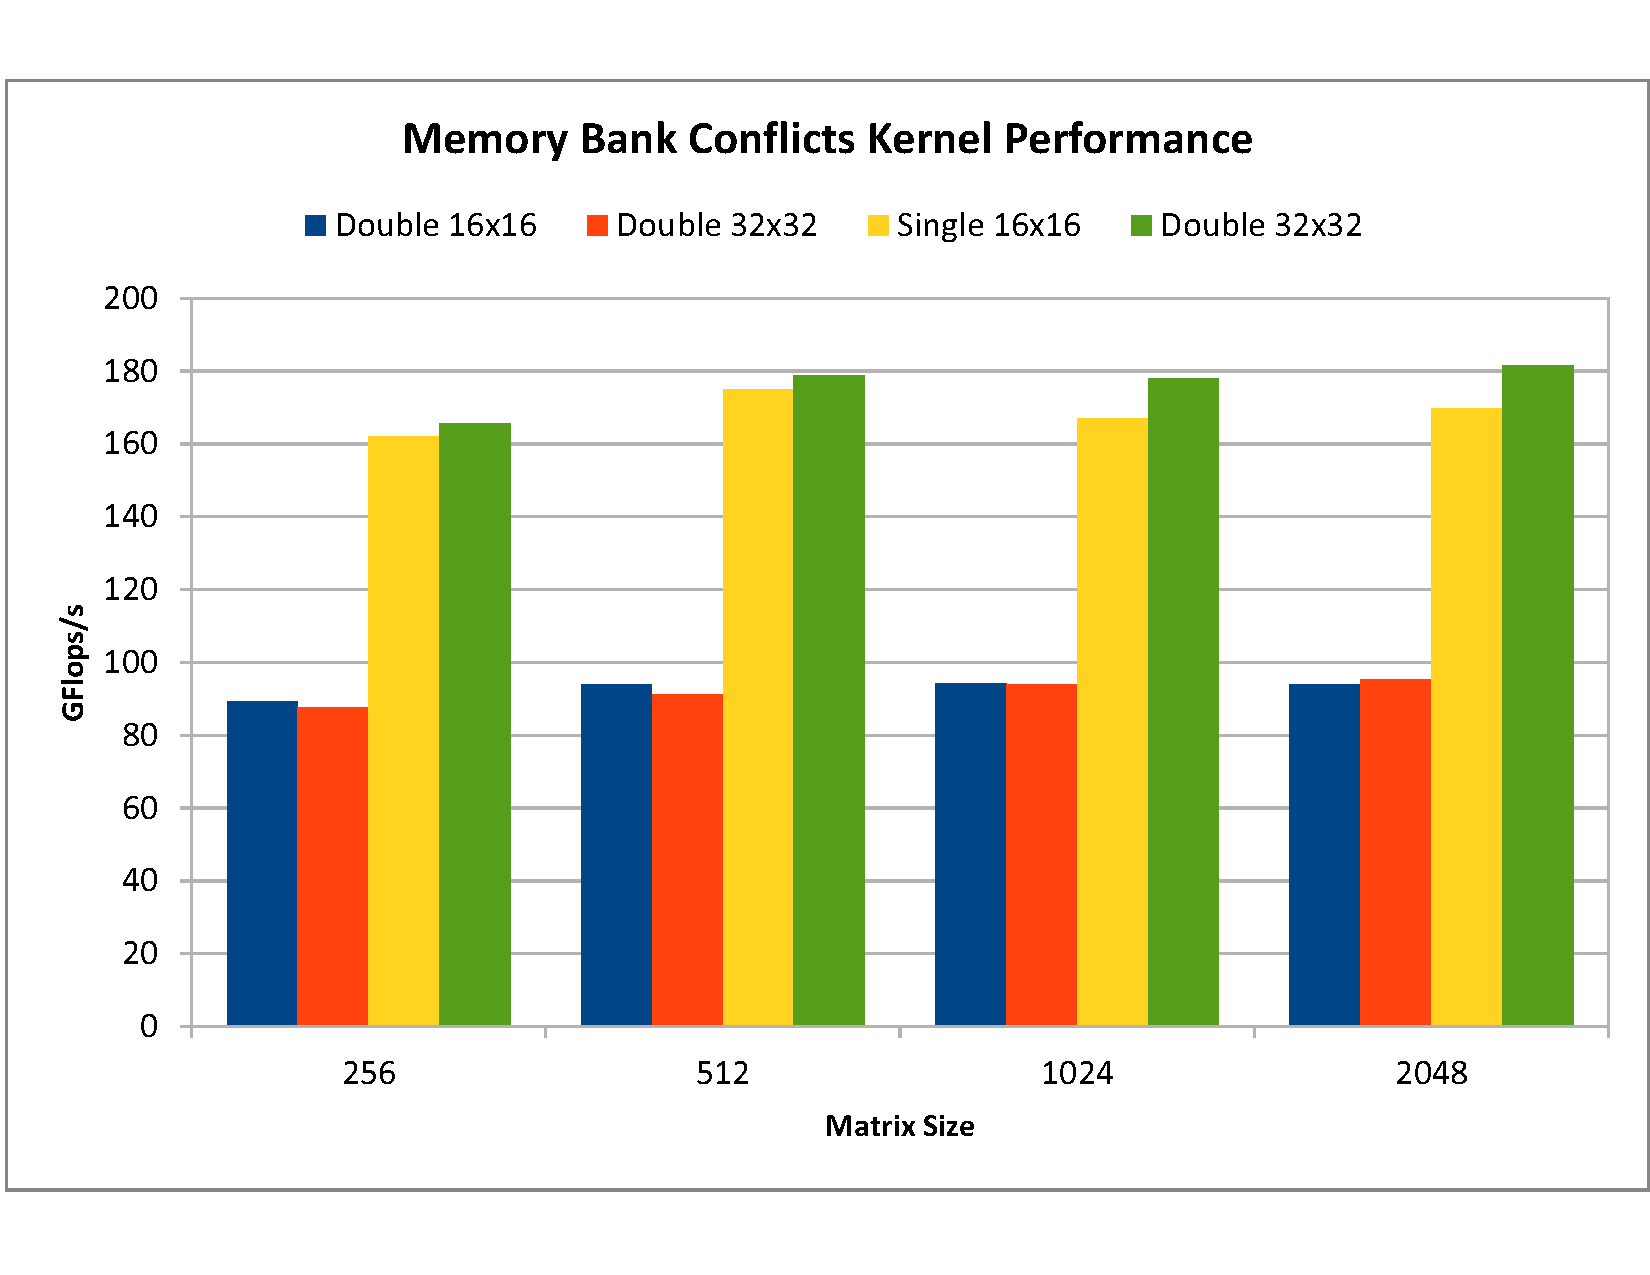
\includegraphics[width=.97\linewidth]{figures/conflicts.pdf}
  \label{fig:conflicts}
\end{subfigure}%
\begin{subfigure}{.5\textwidth}
  \centering
  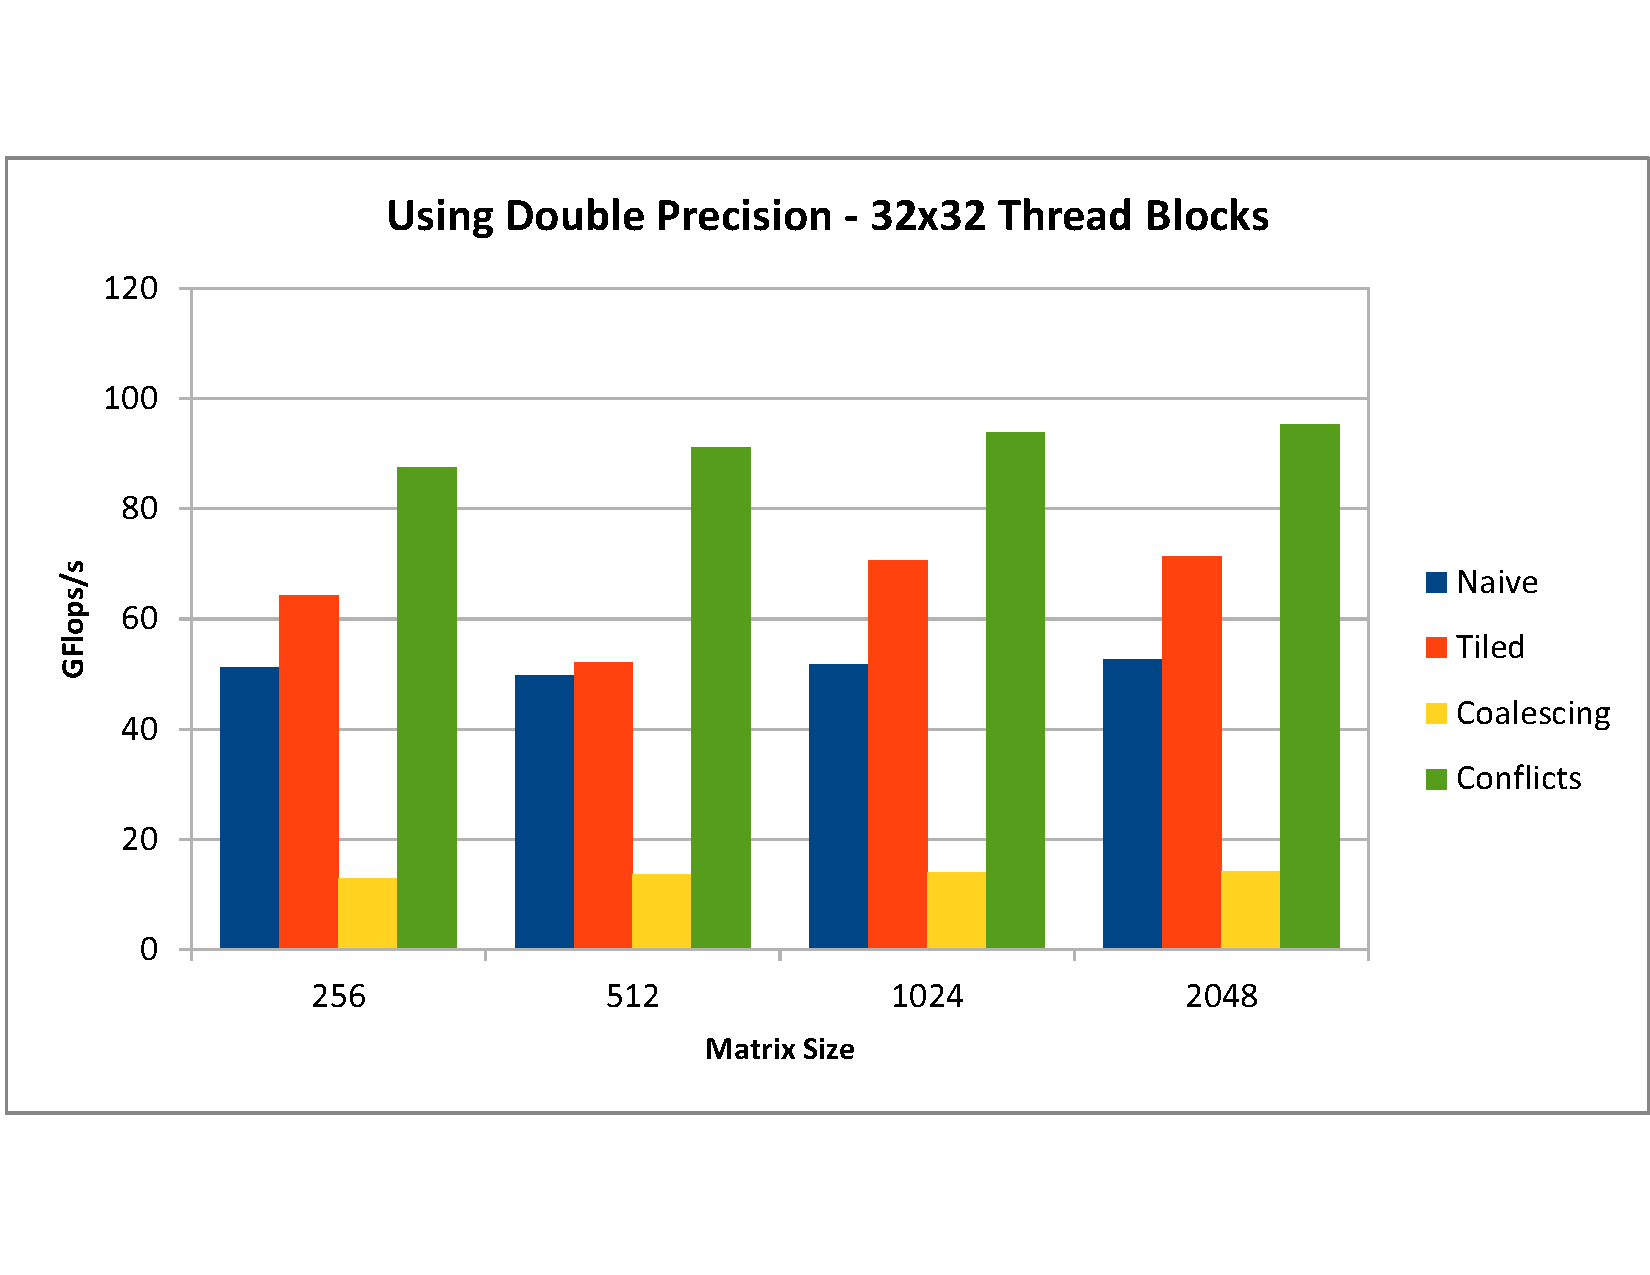
\includegraphics[width=1.03\linewidth]{figures/conflicts_vs_coalescing.pdf}
  \label{fig:conflicts_vs_coalesced}
\end{subfigure}
\caption{Left: The performance of the Bank-Conflict-Avoiding Kernel. Right: This kernel compared against all previous optimizations.}
\label{fig:multi5}
\end{figure}

As shown in Figure \ref{fig:multi5} (left) dealing with bank conflicts significantly improves performance, not just over the coalesced kernel, but over the tiled kernel as well. Figure \ref{fig:multi5} (right) plots all performance measurements up to this point.\\

\section{\textbf{Multiply--Add Balancing}}

Our code includes an expression of the form $C\_temp = C\_temp + (A[i][k] * B[k][j])$. NVidia's Fermi architecture includes fused multiply-add units which theoretically could perform the computation in one step. However, the latest optimization performed so far, stores both A and B into the shared memory and Fermi can only have up to one operand in memory. Consequently, the above computation breaks into a load of either A or B element into one  register and then a fused multiply add instruction. Through the multiply--add balancing optimization, we attempted to store one of the two matrices (particularly B) in registers instead of the shared memory. Under this optimization, the above instruction should be able to perform in one fused multiply-add operation without requiring a load.\\

The first issue is that both A and B are required to be stored in shared memory to efficiently compute the inner product. One solution is to store B in registers and perform outer product. Each thread will multiply each element of a row of A with just the corresponding element of the row of B. The result of each multiplication is added to an individual temporary variable (again stored in registers) and when all the threads of the block complete their execution, each of them is responsible for writing a ``chunk'' of values back to the C matrix.\\

\begin{figure} [h]
\centering
\begin{subfigure}{.5\textwidth}
  \centering
  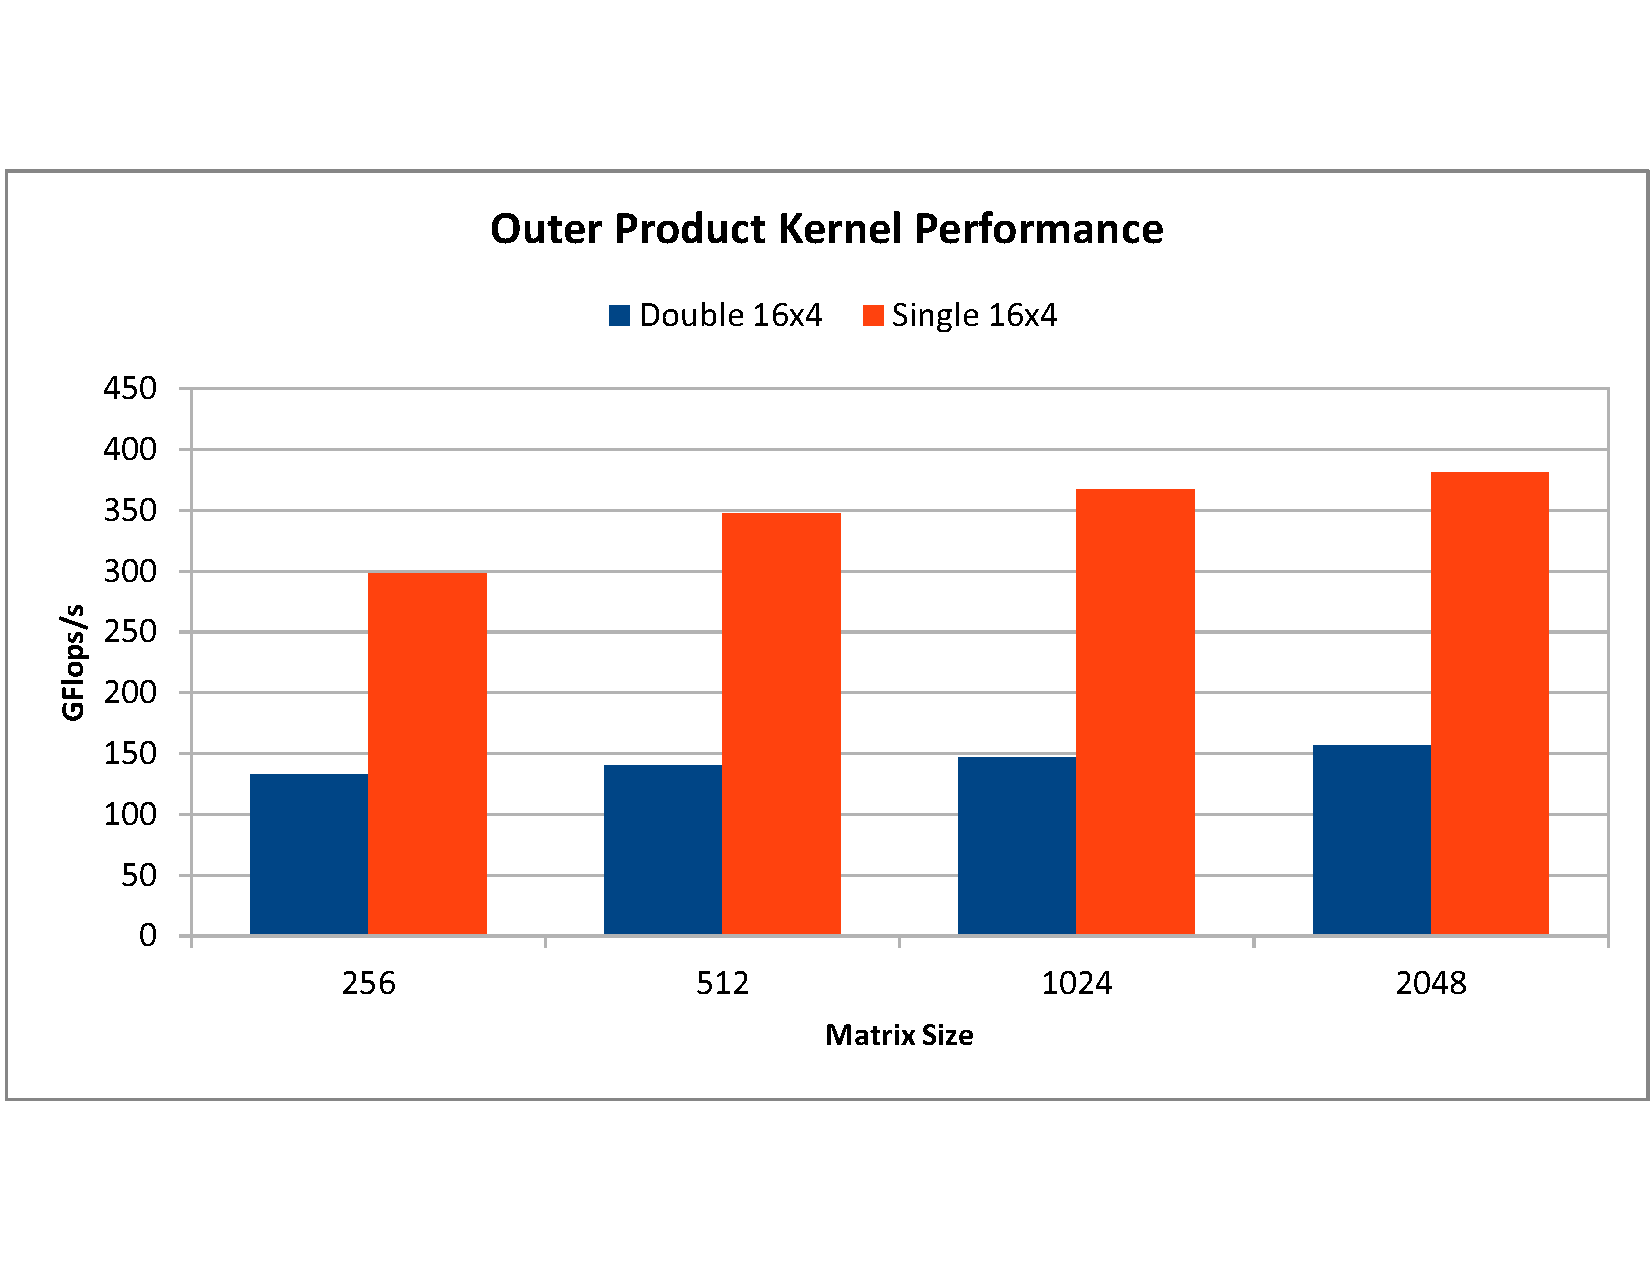
\includegraphics[width=\linewidth]{figures/outer.pdf}
  \label{fig:balancing}
\end{subfigure}%
\begin{subfigure}{.5\textwidth}
  \centering
  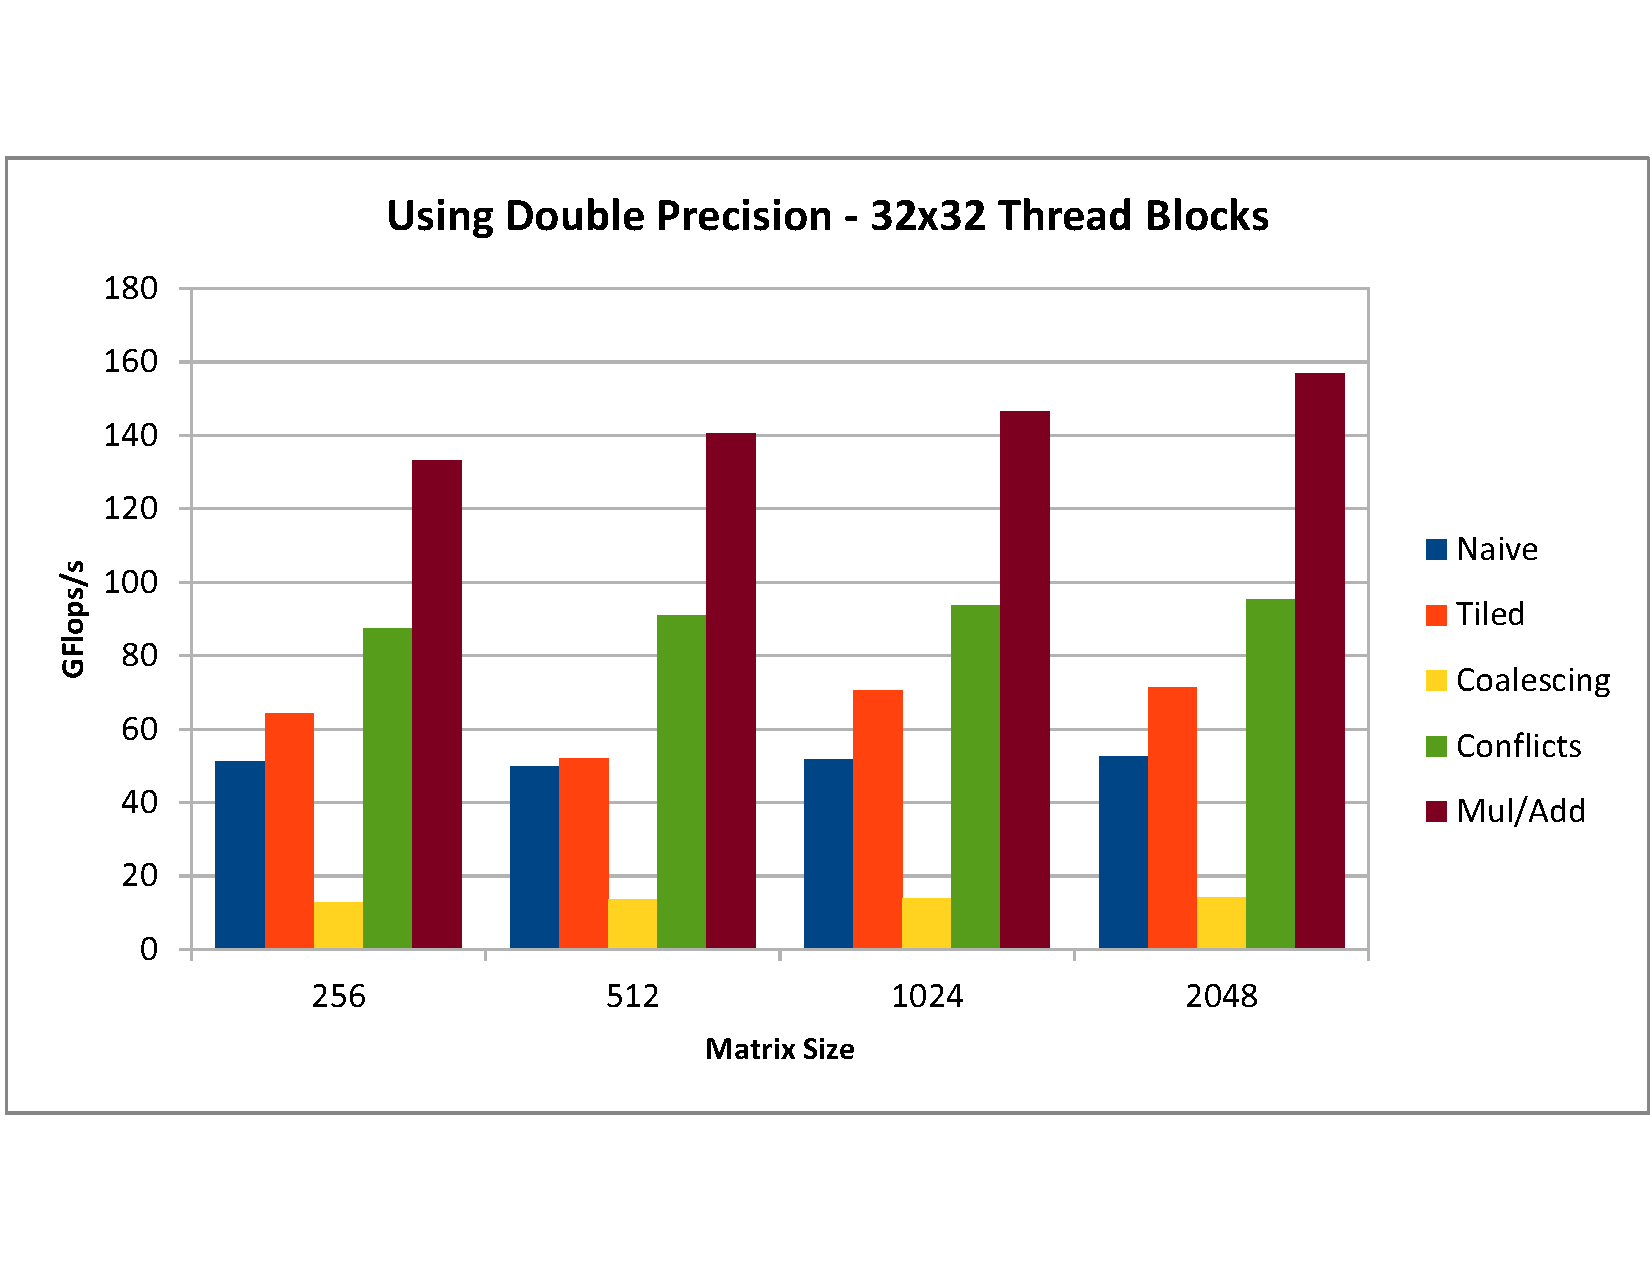
\includegraphics[width=\linewidth]{figures/outer_vs_conflicts.pdf}
  \label{fig:balancing_vs_conflicts}
\end{subfigure}
\caption{Left: The performance of the Multiply-Add Balancing Kernel. Right: This kernel compared against all previous optimizations.}
\label{fig:multi6}
\end{figure}

To better utilize the provided registers, the tile sizes (and the block geometry) were modified for this optimization. The sub-block of A remains 16$\times$16 as it was, but B's tile is now 16$\times$64. When the two tiles are multiplied, the result is a 16$\times$64 tile that will be stored in C. We want each thread to be responsible for calculating one column of C, thus we need blocks of 64 threads (for 64 columns).\\

We programmed the geometry of thread blocks to be 16$\times$4 to provide the required 64 threads. Each of the 4 ``y-threads'' is responsible for loading four elements of A into shared memory, which means that each of the ``x-threads'' is responsible for loading one row of the A sub-block in shared memory. For the computation part, each thread takes a row of A and multiplies each of its element with one element of B at a time. Then it takes the next row of A and the next element of B and repeats. After 16 iterations, the thread has calculated one column of the C tile.\\

Due to the new geometry of our blocks and the new behavior of each thread, we had to modify the geometry of the grid as well. Specifically, the number of blocks in the X-dimension now need to be N/64 and on the Y-direction N/16. These numbers cannot be modified anymore, since the behavior of each thread is now hardcoded into the kernel function. And of course, like the previous cases, N now has to be divisible by 64.\\

Figure \ref{fig:multi6} (left) demonstrates the tremendous performance improvement obtained by this optimization, while Figure \ref{fig:multi6} (right) overlays all measured performances up to this point. The following optimizations (prefetching and loop-unrolling) are built on top of this optimization.

\section {\textbf{Prefetching}}
Prefetching is a very well known optimization technique when handling memory-bound workloads. Essentially, prefetching means to bring certain values closer to the processor in expectation of their use. We modified our kernel in order to load the required values from the A matrix into "prefetch" arrays ahead of the time these values will be used. The main operation remains the same as the multiply-add optimization.\\

\begin{figure} [h]
\centering
\begin{subfigure}{.5\textwidth}
  \centering
  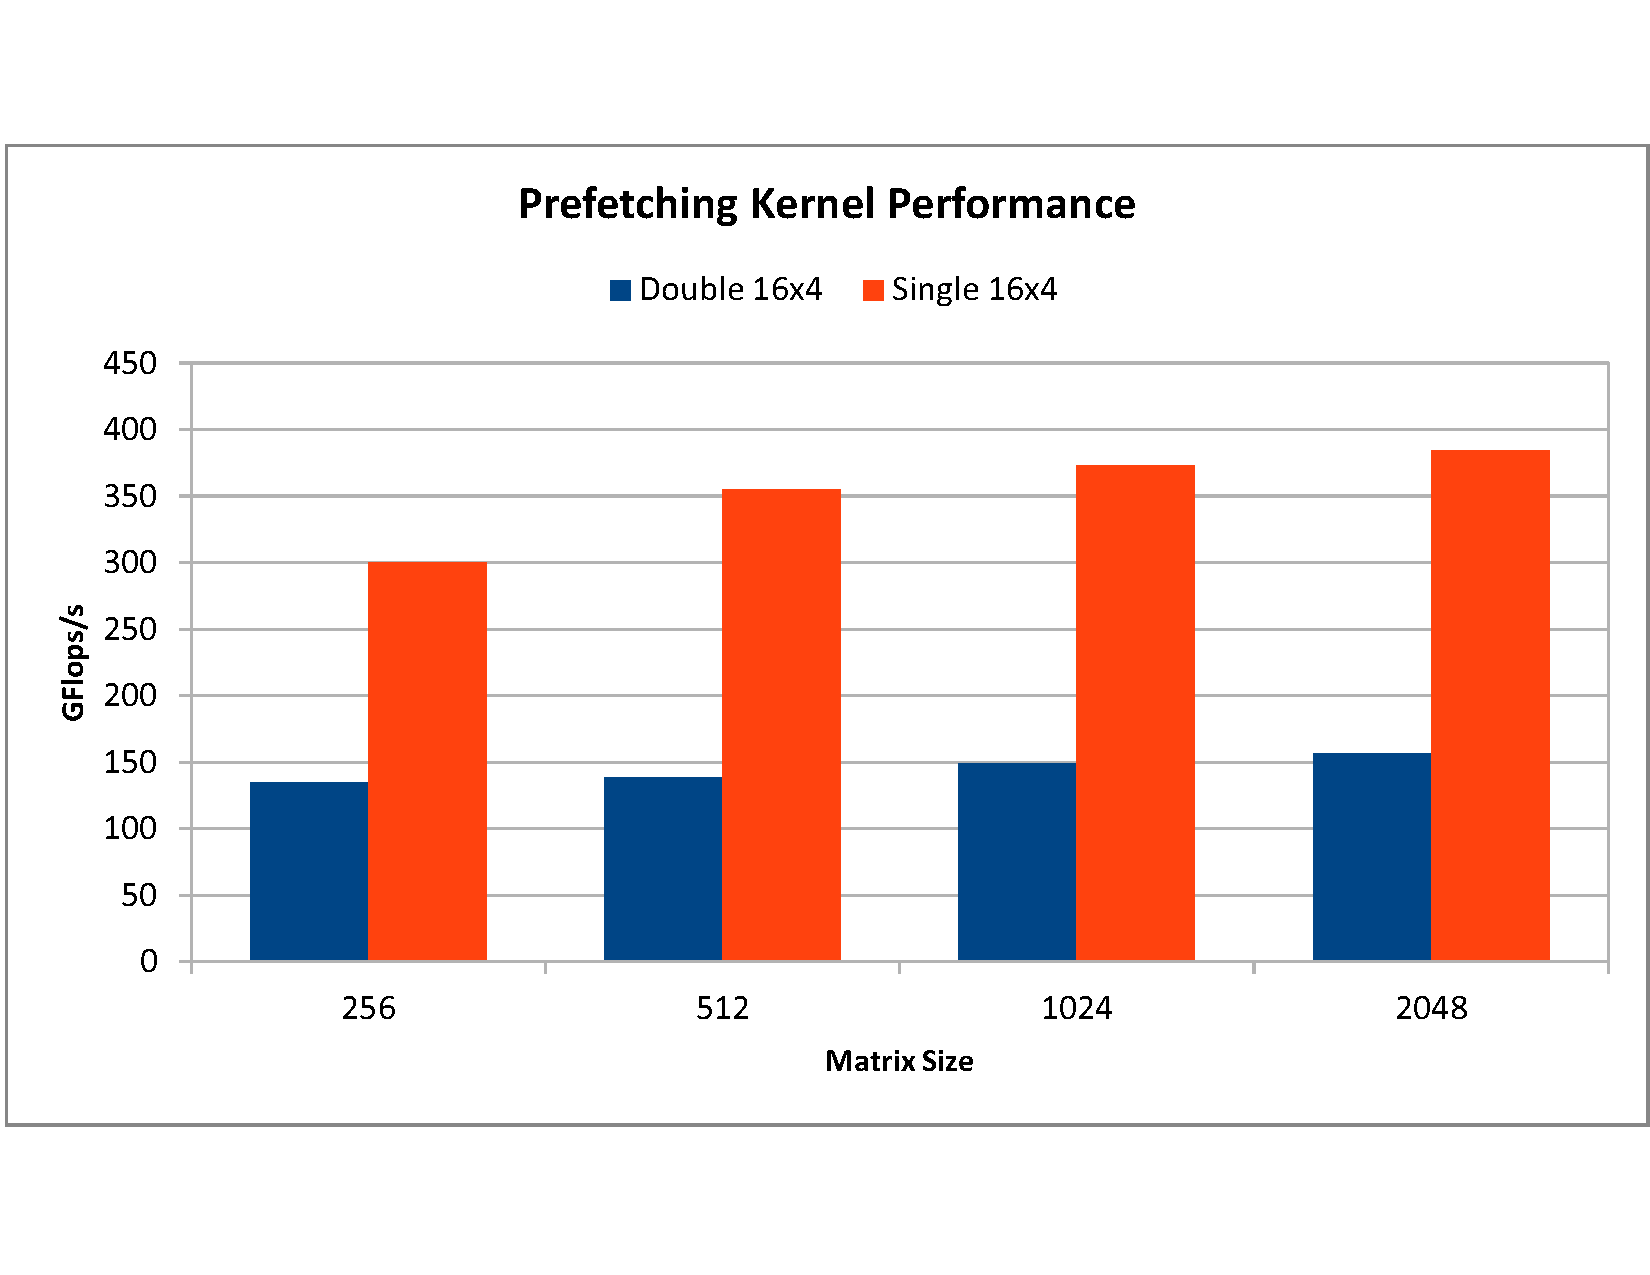
\includegraphics[width=\linewidth]{figures/prefetch.pdf}
  \label{fig:prefetch}
\end{subfigure}%
\begin{subfigure}{.5\textwidth}
  \centering
  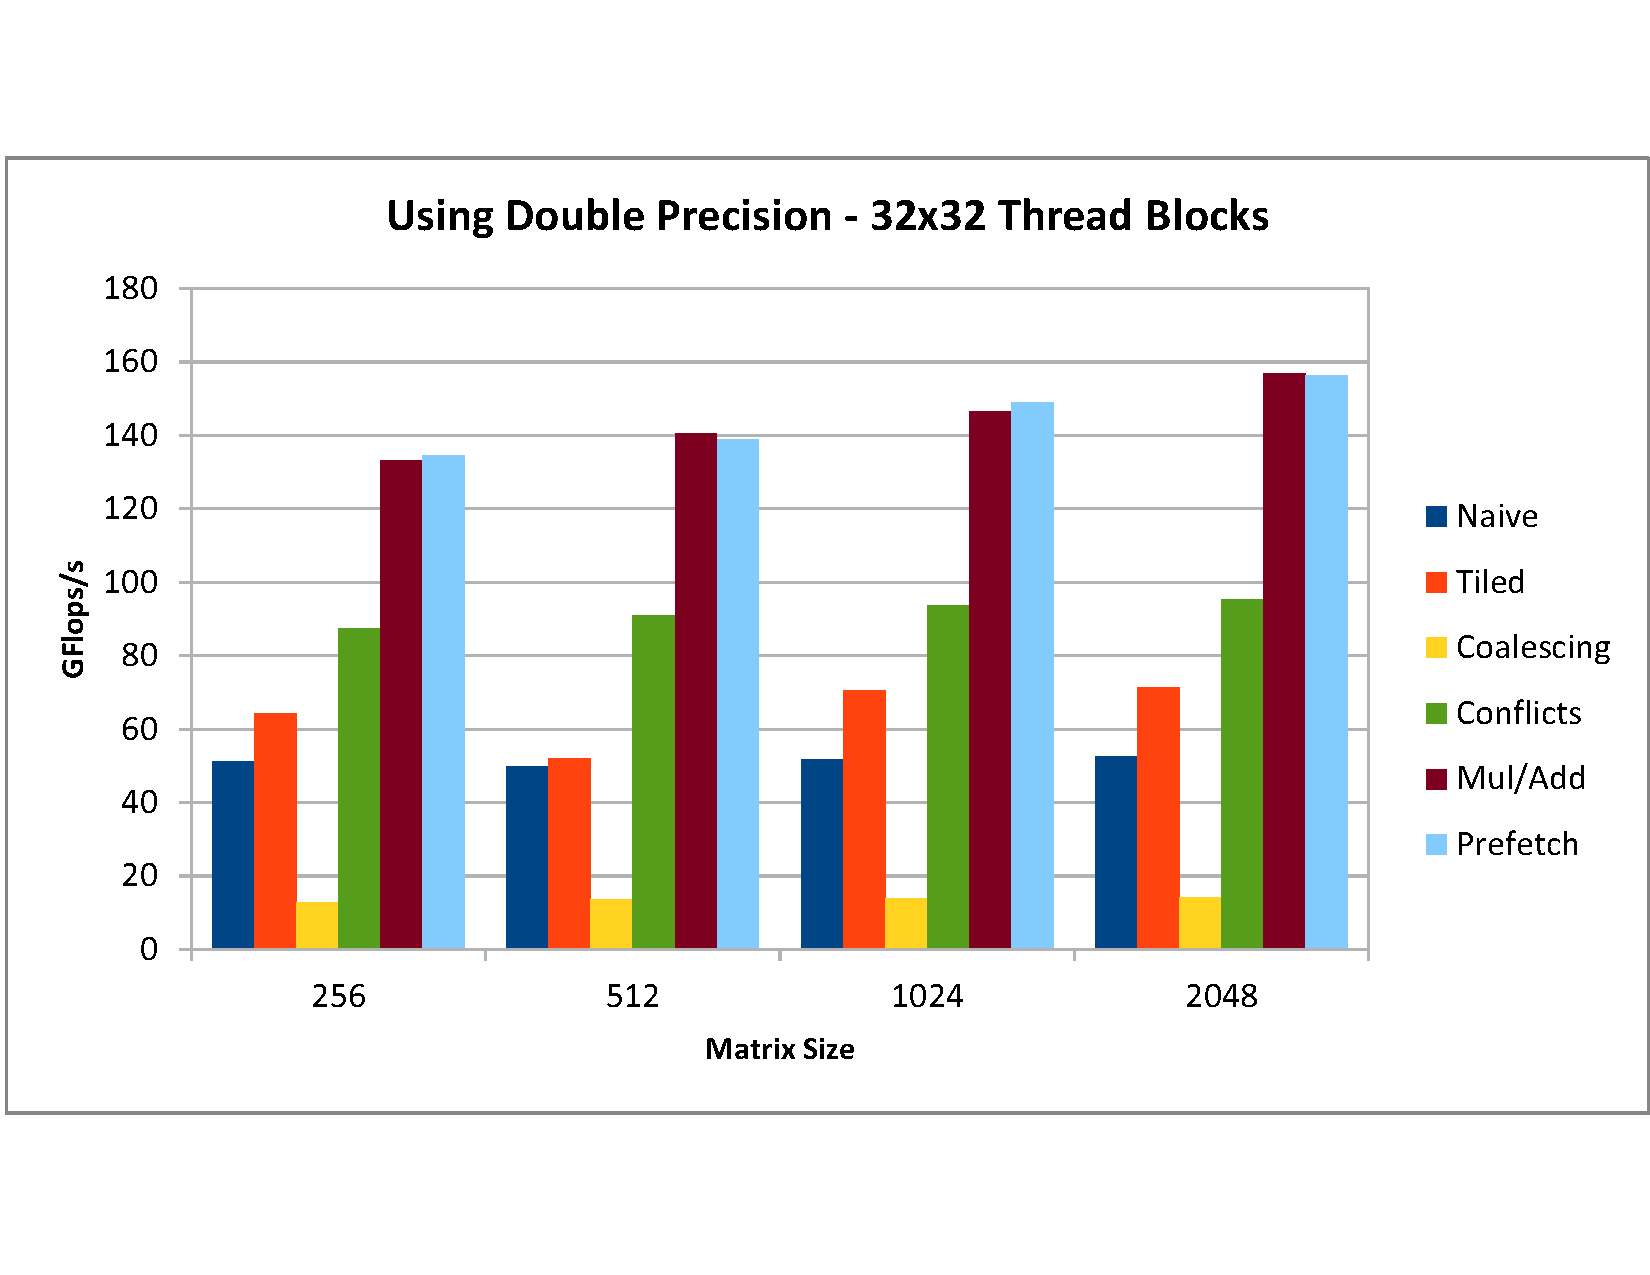
\includegraphics[width=\linewidth]{figures/prefetch_vs_outer.pdf}
  \label{fig:prefetch_vs_balancing}
\end{subfigure}
\caption{Left: The performance of the Prefetching Kernel. Right: Prefetching kernel compared against all previous optimizations.}
\label{fig:multi7}
\end{figure}

Figures \ref{fig:multi7} (left) and \ref{fig:multi7} (right) demonstrate the performance improvement with prefetching.\\

\section{\textbf{Unrolling}}
\begin{figure} [h]
\centering
\begin{subfigure}{.5\textwidth}
  \centering
  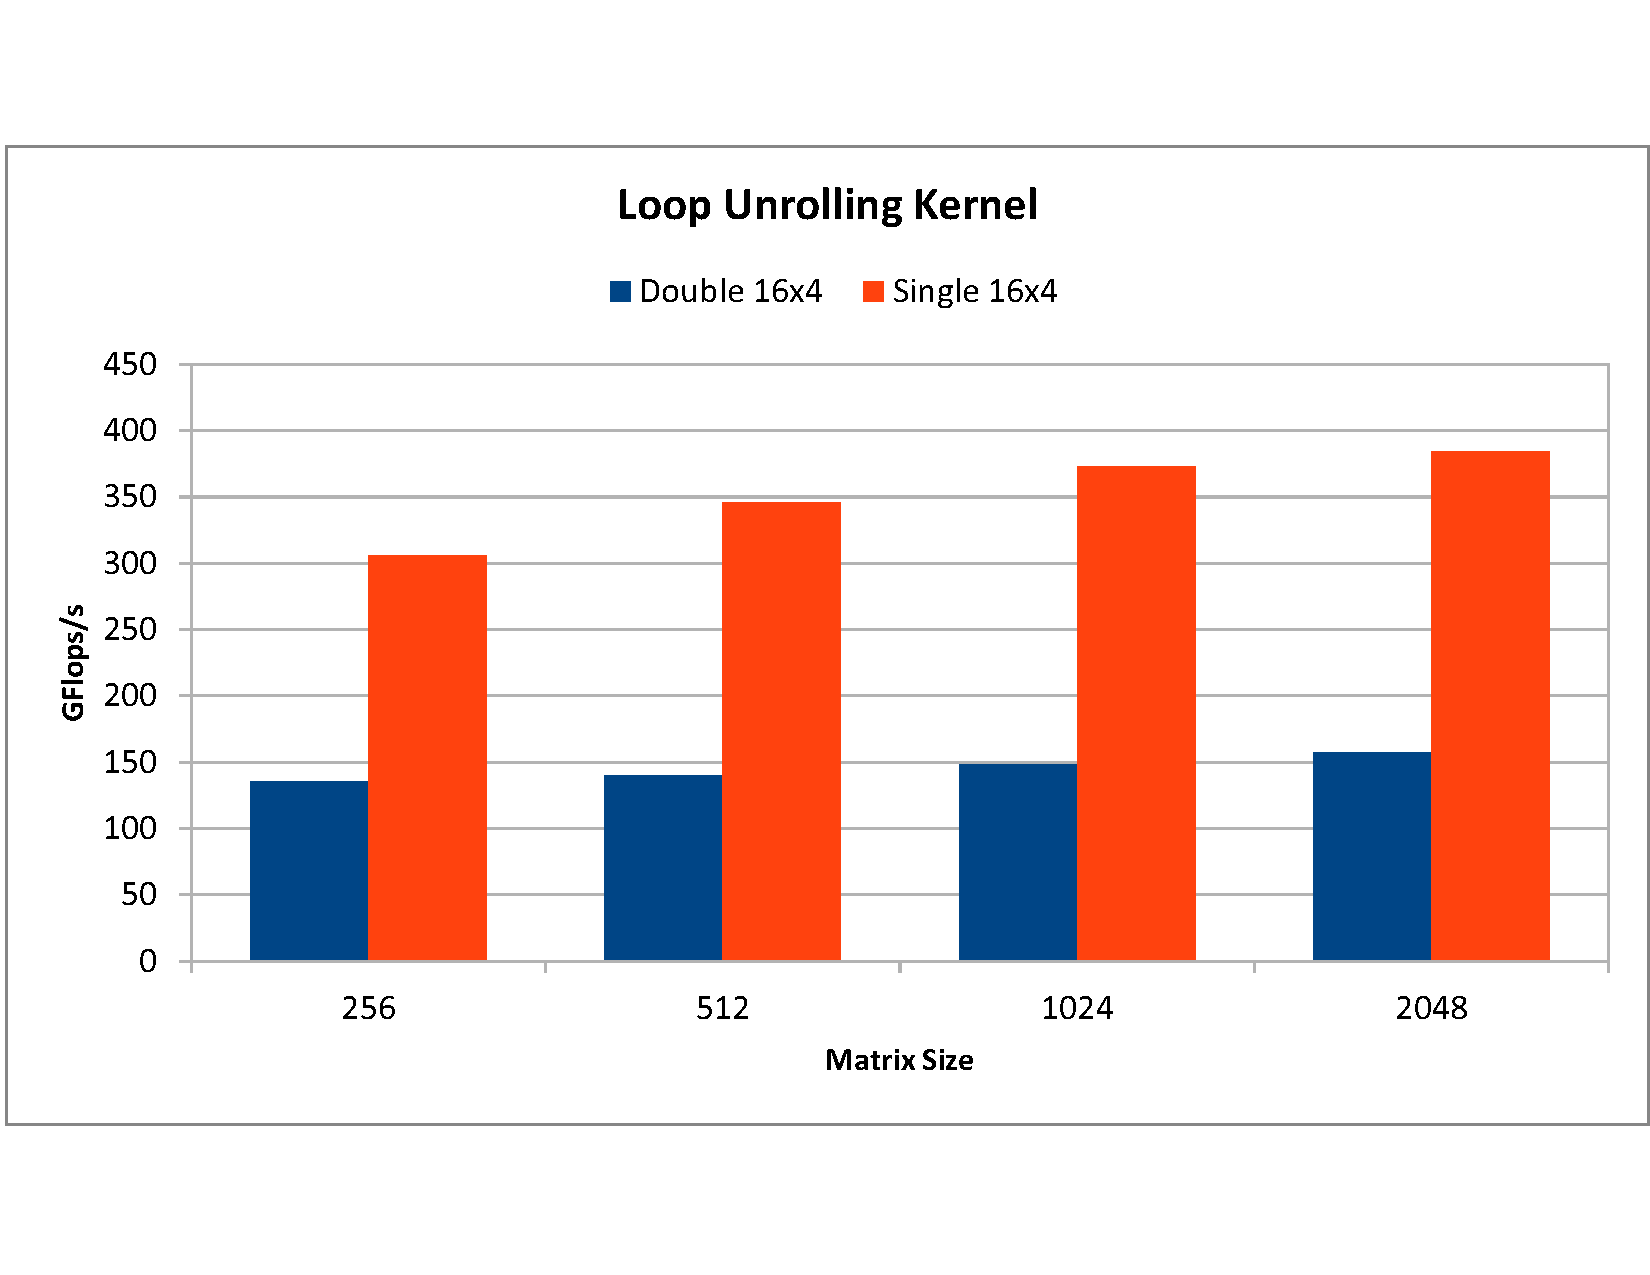
\includegraphics[width=\linewidth]{figures/unrolling.pdf}
  \label{fig:unroll}
\end{subfigure}%
\begin{subfigure}{.5\textwidth}
  \centering
  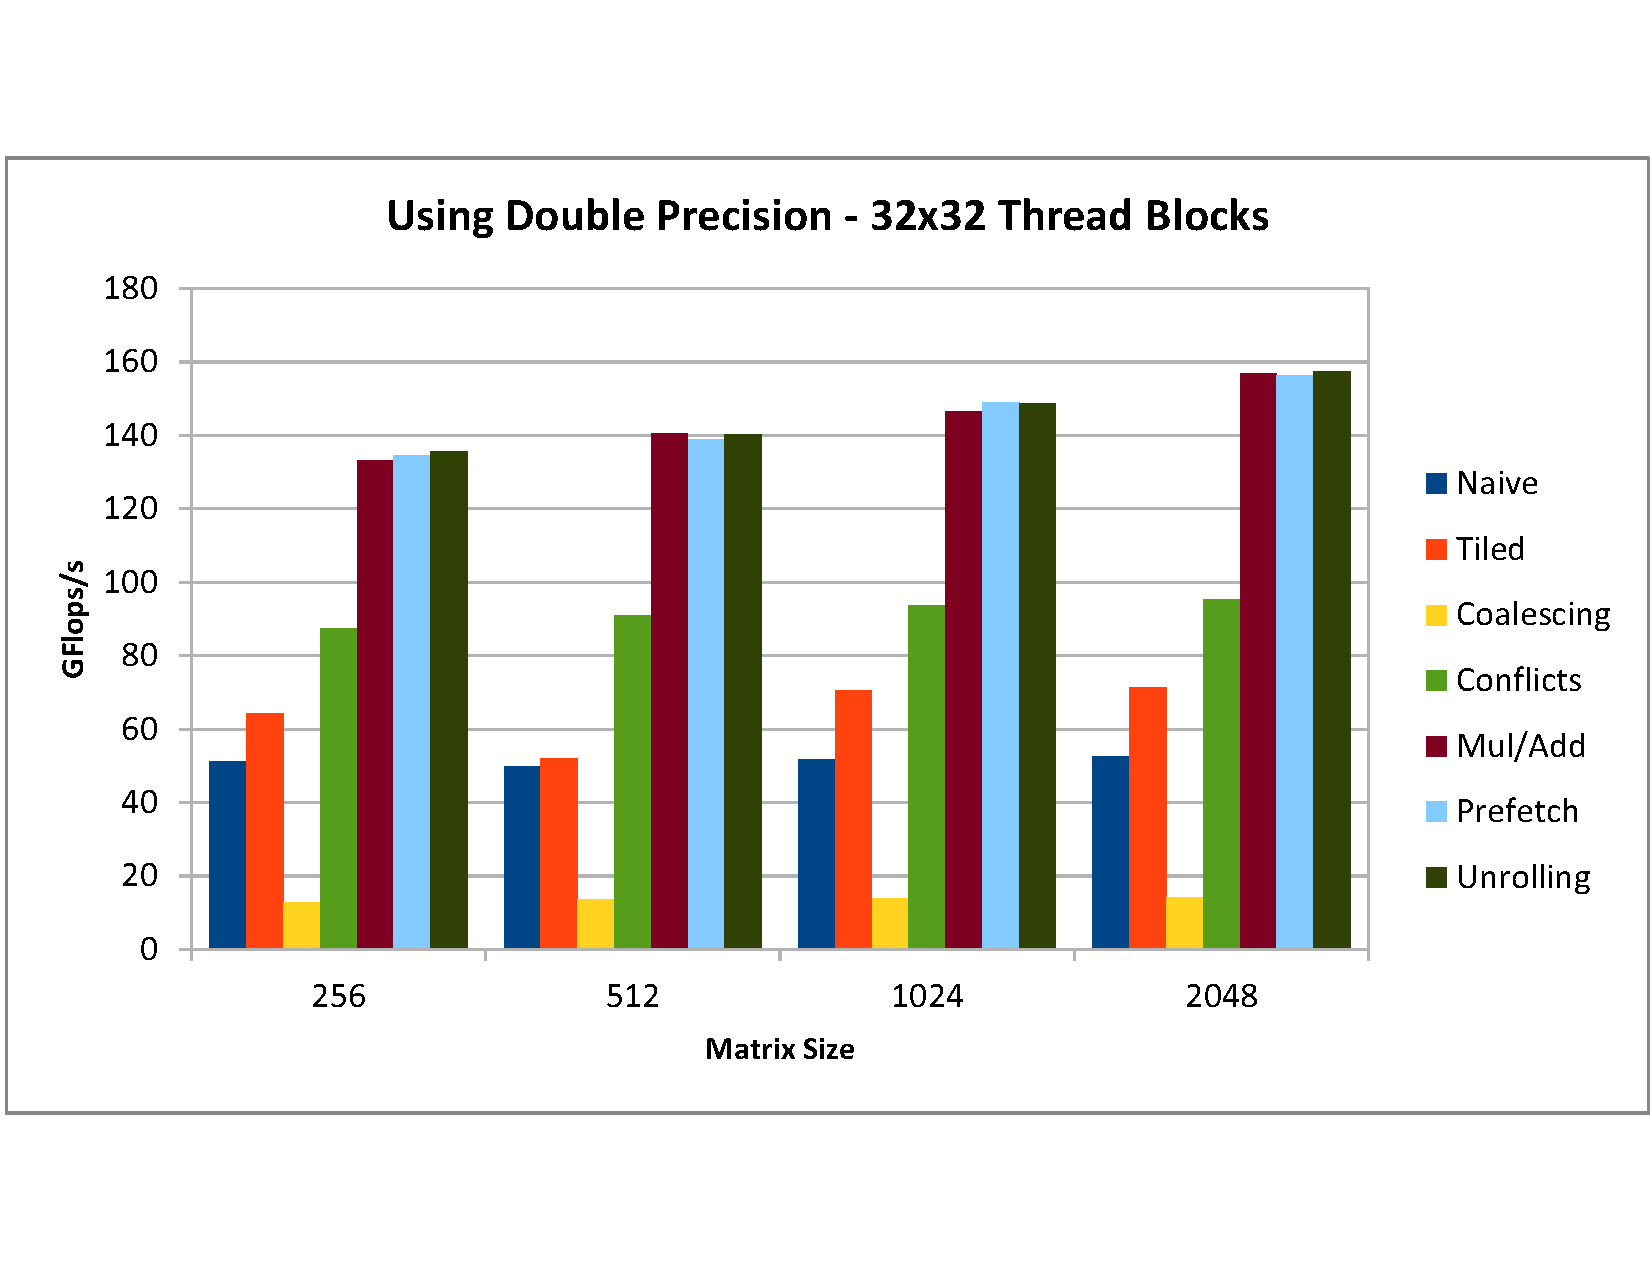
\includegraphics[width=\linewidth]{figures/unrolling_vs_prefetch.pdf}
  \label{fig:unroll_vs_prefetch}
\end{subfigure}
\caption{Left: The performance of the Loop Unrolling Kernel. Right: This kernel compared against all previous optimizations.}
\label{fig:multi8}
\end{figure}

As a final optimization, we tried to use ``\#pragma unroll'' to order the compiler to unroll the loops of our kernel function. As a result, we were able to decrease the loop overhead imposed.\\



\section{\textbf{Conclusions}}
For this assignment we were asked to optimize matrix multiplication for NVIDIA's Fermi GPU. Through a series of six optimizations we were able to improve the performance from ~25 GFlops/s that the naive implementation would report, up to ~150 GFlops/s. Some of the optimizations actually hurt -- and in some cases significantly -- the performance, leading to interesting observations about the underlying hardware and our program's behavior.

\end{document}
